\documentclass[russian,utf8,emptystyle]{eskdtext}

\usepackage[T2A,T1]{fontenc}

\newcommand{\No}{\textnumero} % костыль для фикса ошибки

\ESKDdepartment{Федеральное государственное бюджетное образовательное учреждение высшего профессионального образования}
\ESKDcompany{Московский государственный технический университет им. Н. Э. Баумана}
\ESKDclassCode{23 0102}
\ESKDtitle{Подсистема работы с текстовыми данными на географической карте «Волхв-Гео»}
\ESKDdocName{Расчетно-пояснительная записка}
\ESKDauthor{Оганян~Л.~П.}
\ESKDtitleApprovedBy{~}{~\underline{\hspace{2.5cm}}}
\ESKDtitleAgreedBy{~}{~\underline{\hspace{2.5cm}}}
\ESKDtitleDesignedBy{Студент группы ИУ5-122}{Оганян~Л.~П.}

\usepackage{multirow}
\usepackage{tabularx}
\usepackage{tabularx,ragged2e}
\usepackage{pdfpages}
\renewcommand\tabularxcolumn[1]{>{\Centering}p{#1}}
\newcommand\abs[1]{\left|#1\right|}

\usepackage{longtable,tabu}

\usepackage{geometry}
\geometry{footskip = 1cm}

\pagenumbering{arabic}
\pagestyle{plain}

\usepackage{setspace}

\usepackage{xcolor}
\usepackage{listings}
\lstset{
    breaklines=true,
    postbreak=\raisebox{0ex}[0ex][0ex]{\ensuremath{\color{red}\hookrightarrow\space}},
    extendedchars=\true,
    basicstyle=\small,
    inputencoding=utf8,
    numbers=left,                    
    numbersep=5pt,                  
    numberstyle=\tiny\color{mygray}
}

\renewcommand{\lstlistingname}{Листинг}
\renewcommand{\lstlistlistingname}{Листинги}

\ESKDsectAlign{section}{Center} % to capitalize russian text

\usepackage{array}
\newcolumntype{L}[1]{>{\raggedright\let\newline\\\arraybackslash\hspace{0pt}}m{#1}}
\newcolumntype{C}[1]{>{\centering\let\newline\\\arraybackslash\hspace{0pt}}m{#1}}
\newcolumntype{R}[1]{>{\raggedleft\let\newline\\\arraybackslash\hspace{0pt}}m{#1}}

\usepackage{tikz}
\usepackage{pgf-pie}

\usepackage{totcount}
\regtotcounter{figure}
\regtotcounter{table}

\usepackage{hyperref}

\setcounter{secnumdepth}{5}
\setcounter{tocdepth}{5}

%\renewcommand*{\thesection}{\arabic{section}}

%===========================================================================
\begin{document}

\clearpage
\clearpage

\section*{Реферат}

Данная расчетно-пояснительная записка содержит \pageref{LastPage} (без приложения) страниц, \total{figure} иллюстраций (без приложения), \total{table} таблиц, 2 приложения, ?? использованных источников.

Ключевые слова: полнотекстовый поиск, сбор информации, формальный язык запросов, генетическое программирование, эволюционные алгоритмы, символьная регрессия, анализ временных рядов, геоинформационная система.

Данный дипломный проект посвящен разработке подсистемы анализа новостных потоков в текстовом виде, прогнозирования их активности и отображения на географической карте. Целью разработки является обработка собранной из открытых источников информации, выделение географически ограниченных тем новостей, анализ новостной динамики, визуализация полученных данных на географической карте, построение аналитических заметок на основе полученных данных.

Подсистема проектируется в виде веб-сервиса, предоставляющего пользователю набор экранных форм для взаимодействия с данным программных изделием, а также машинный интерфейс для взаимодействия стороннего программного обеспечения с данной подсистемой. Структуру подсистемы составляют сервер приложения, сервер СУБД, сервер индексации и терминалы пользователей. При разработке программного продукта используется язык программирования Haskell.

В результате разработки была спроектирована подсистема, отвечающая требованиям технического задания и имеющая возможности, необходимые как для всестороннего анализа новостной информации, так и для наглядного отображения её на географической карте. 

Область применения подсистемы -- аналитические центры, лаборатории анализа данных, новостные и политические агенства, органы государственной власти.

Проект является некоммерческим с малой стоимостью выполнения.

\tableofcontents

\section*{Нормативные ссылки}

В дипломном проектировании использованы следующие стандарты:
\begin{itemize}
\item ГОСТ 2.105-95 -- «ЕСКД. Общие требования к текстовым документам».
\item ГОСТ 7.1-2003  -- «СИБИД. Библиографическая запись. Библиографическое описание. Общие требования и правила составления».
\item ГОСТ 7.12-93 -- «СИБИД. Библиографическая запись. Сокращение слов на русском языке».
\item ГОСТ 7.32-2001 -- «СИБИД. Отчет о научно-исследовательской работе. Структура и правила оформления».
\item ГОСТ 19.701-90 -- «ЕСКД. Схемы алгоритмов, программ, данных и систем. Условные обозначения и правила выполнения».
\item ISO 3166 -- <<Кодовые обозначения государств и зависимых территорий, а также основных административных образований внутри государств>>
\item СанПиН 2.2.1/2.1.1.1278-03 -- «Гигиенические требования к естественному, искусственному и совмещенному освещению жилых и общественных зданий».
\item СанПиН 2.2.2/2.4.1340-03 -- «Гигиенические требования к видеодисплейным терминалам, персональным электронно-вычислительным машинам и организации работы».
\item СНиП 2.04.05-86  --  «Отопление, вентиляция и кондиционирование».
\end{itemize}

В расчетно-пояснительной записке имеются ссылки на следующие стандарты:
\begin{itemize}
\item ГОСТ 12.1.002-84 -- «ССБТ. Электрические поля промышленной частоты. Допустимые уровни напряженности и требования к проведению контроля на рабочих местах».
\item ГОСТ 12.1.003-83 -- «ССБТ. Шум. Общие требования безопасности».
\item ГОСТ 12.1.004-91 -- «ССБТ. Пожарная безопасность. Общие требования».
\item ГОСТ 12.1.005-88 -- «ССБТ. Общие санитарно-гигиенические требования к воздуху рабочей зоны».
\item ГОСТ 12.1.006-84 -- «ССБТ. Электромагнитные поля радиочастот. Допустимые уровни на рабочих местах и требования к проведению контроля».
\item ГОСТ 12.2.007.3-75 -- «ССБТ. Электротехнические устройства на напряжение свыше 1000 В. Требования безопасности».
\item ГОСТ 12.2.007.4-75 -- «ССБТ. Шкафы комплектных распределительных устройств и комплектных трансформаторных подстанций, камеры сборные одностороннего обслуживания, ячейки герметизированных элегазовых распределительных устройств».
\item ГОСТ 12.1.010-76 -- «ССБТ. Взрывобезопасность. Общие требования».
\item ГОСТ 12.1.018-93 -- «ССБТ. Пожаровзрывобезопасность статического электричества. Общие требования».
\item ГОСТ 12.1.038-82 -- «ССБТ. Электробезопасность. Предельно допустимые значения напряжений прикосновения и токов».
\item ГОСТ 12.1.045-84 -- «ССБТ. Электростатические поля. Допустимые уровни на рабочих местах и требования к проведению контроля».
\item ГОСТ 12.4.124-83 -- «ССБТ. Средства защиты от статического электричества. Общие технические требования».
\item СанПиН 2.2.4.548-96 -- «Гигиенические требования к микроклимату производственных помещений».
\item СНиП 23-05-95 -- «Естественное и искусственное освещение».
\end{itemize}
\section*{Определения, обозначения и сокращения}

\begin{itemize}
\item АИС -- автоматизированная информационная система.
\item АПК -- аппаратно-программный комплекс.
\item БД -- база данных.
\item ЕСКД -- единая система конструкторской документации.
\item Управляющий класс (control) -- класс модели анализа, представляющий координацию, последовательность и управление другими объектами, часто используется для инкапсуляции управления для варианта использования.
\item Граничный класс (boundary) -- класс модели анализа, используемый для моделирования взаимодействия между системой и ее актантами, то есть пользователями и внешними системами.
\item Класс сущности (entity) -- класс модели анализа, используемый для моделирования долгоживущей, часто персистентной информации.
\item ОЗУ -- оперативное запоминающее устройство.
\item ОС -- операционная система.
\item ПК -- персональный компьютер.
\item ПО -- программное обеспечение.
\item ПЭВМ -- персональная электронно-вычислительная машина.
\item СанПиН -- санитарно-эпидемиологические правила и нормативы.
\item СИБИД -- система стандартов по информации, библиотечному и издательскому делу.
\item СНиП -- строительные нормы и правила. 
\item ССБТ -- система стандартов по информации, библиотечному и издательскому делу.
\item СУБД -- система управления базами данных.
\item ЭВМ -- электронно-вычислительная машина.
\item ЭМП -- электромагнитное поле.
\item API -- application programming interface -- набор готовых классов, процедур, функций, структур и констант, предоставляемых приложением (библиотекой, сервисом) для использования во внешних программных продуктах.
\item CPU -- central processing unit -- центральный процессор.
\item HDD -- hard disk drive -- жесткий диск.
\item SQL -- structured query language -- универсальный компьютерный язык, применяемый для создания, модификации и управления данными в реляционных базах данных. SQL основывается на исчислении кортежей. SQL является, прежде всего, информационно-логическим языком, предназначенным для описания, изменения и извлечения данных, хранимых в реляционных базах данных. 
\item UML -- unified modeling language, унифицированный язык моделирования -- язык графического описания для объектного моделирования в области разработки программного обеспечения. UML является языком широкого профиля, это открытый стандарт, использующий графические обозначения для создания абстрактной модели системы, называемой UML-моделью.
\end{itemize}
\section*{Введение}

Дипломный проект на тему <<Автоматизированная информационная система отслеживания и прогнозирования новостных потоков <<Волхв>> >> посвящен созданию системы, которая позволит накапливать информацию из открытых источников СМИ, аналитических материалов экспертов, социальных сетей, а также предоставит инструменты для всестороннего анализа накопленной информации. АИС <<Волхв>> предоставляет два способа анализа накопленной новостной информации: с помощью проблемно-ориентированного языка запросов и с помощью автоматизированного прогнозирования количества сообщений, удовлетворяющих заданному запросу.



%===========================================================================
% Конструкторская часть
\section{Конструкторская часть}

\subsection{Постановка задачи проектирования}

Подсистема работы с текстовыми данными на географической карте <<Вохв-ГЕО>> позволяет проводить накопление и анализ новостных документов с помощью формализованного языка запросов для отображения на карте. Данная подсистема предназначена для исследовательской деятельности и для включения в состав сложных комплексов анализа событий в новостных потоках.

Подсистема «Волхв-ГЕО» должна выполнять следующие функции
\begin{itemize}
\item Удаленный доступ к системе. Программное изделие должно обеспечивать удаленный доступ к системе через Web-сервер.
\item Соединение с базой данных. Программное изделие должно осуществлять удаленное соединение с базой данных.
\item Ввод с клавиатуры. Данные, вводимые с клавиатуры должны иметь тип и формат, соответствующий типу и формату полей записи.
\item Добавление информации в базу данных. Программное изделие должно осуществлять добавление новой записи в базу данных при условии, что эта запись удовлетворяет всем требованиям, налагаемым на входные данные.
\item Удаление информации из базы данных. Программное изделие должно осуществлять исключение выбранной пользователем записи в таблице из исходной базы данных.
\item Редактирование информации в базе данных. Функция должна осуществлять редактирование поля записи, выбранного пользователем. При этом при редактировании данных должны выполняться все требования, налагаемые на входные данные.
\item Геопривязка новостей.
\item Анализ динамики новостей.
\item Отображение данных на карте. Функция должна осуществлять отображение новостной информации на карте.
\item Создание сценариев. Функция должна обеспечивать создание и редактирование сценария – набора визуальных элементов на карте.
\item Создание аналитической заметки. Функция должна обеспечивать создание и редактирование аналитической заметки – текстового сопровождения к сценарию
\end{itemize}

%\clearpage
\subsection{Описание предметной области}
\subsubsection{Естественно-языковая модель предметной области}

На данный момент существует очень мало систем, позволяющих проводить работу с новостными данными на географических картах. Ближайшие аналоги предоставляют отображение на карте новостной информации, предоставленной пользователями, собранной и обработанной в ручном режиме.

Подсистема <<Волхв-ГЕО>> должна работать в составе более крупной АИС, обеспечивая отображение собранных новостных данных на карте и должна предоставлять инструментарий по прогнозированию ситуаций и построению аналитических заметок. Подсистема использует формализованные запросы для решения задачи геотегирования текстов: формализованный запрос может определять географические привязки новостных сообщений путем учета упоминаемых географических названий. К результатам такого запроса можно привязать географические метки, чтобы использовать их в более сложных запросах.

Для реализации этой задачи требуется база новостей и система полнотекстового поиска по индексированным документам, которая не входит в структуру проектируемой подсистемы и является внешней системой, обозначаемой ИПС.

Требования, накладываемые на ИПС:
\begin{itemize}
\item Поддержка полнотекстового индекса
\item Поддержка полнотекстовых запросов
\item Поддержка запросов с учётом морфологии языка
\item Поддержка сохранённых запросов
\item Возможность редактирования документов посредством API
\item Поддержка текстовых меток
\end{itemize}

Подсистема Волхв-ГЕО, используя сохранённые в своей базе запросы, опрашивает ИПС. Полученные документы помечаются соответствующей геометкой. Используя запросы, сохранённые в ИПС, подсистема Волхв-ГЕО получает документы по требуемым темам и сохраняет агрегированные значения в собственной базе для последующего анализа.
По агрегированным значениям из собственной базы подсистема проводит анализ и результаты анализа сохраняются для дальнейшего использования аналитиком.

Первичной задачей является разметка документов геометками. За исключением случаев, когда координаты места события предоставлены в тексте новости, невозможно в автоматическом режиме точно привязать событие к конкретной точке земной поверхности.

Поэтому представляется нецелесообразным использование в качестве меток географических координат -- широты и долготы. В процессе проектирования было принято решение в качестве минимального географического объекта принять субъекты первого уровня, в рамках подсистемы называемые <<провинциями>>. Например, для Российской Федерации это соответствует субъекту федерации, для США -- штату, для Армении -- марзу.

Согласно стандарту ISO 3166, каждому государству соответствует двух и трёхбуквенный код, а каждому субъекту первого уровня -- код, состоящий из кода страны и кода субъекта.
Код страны/субъекта является текстовой меткой, используемой в подсистеме.

Для провинций, присутствующих в стандарте используется код из стандарта. Для провинций не присутствующих в стандарте, в основном это непризнанные территории, вводится собственное кодовое обозначение по методике, принятой в стандарте.

Результатом работы пользователя в подсистеме является сценарий развития ситуации, и аналитическая записка.

Сценарий представляет из себя набор графических элементов карты с сопроводительным текстом.

Аналитическая записка включает в себя текстовое описание текущей ситуации, сценария развития ситуации и иную информацию по необходимости.

Предметная область разработанной автоматизированной системы представлена на
рисунке~\ref{figure:domain}.

\begin{figure}[!h]
\centering
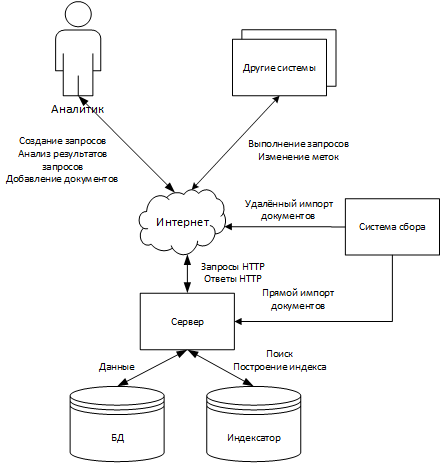
\includegraphics{design/domain}
\caption{Схема предметной области.}
\label{figure:domain}
\end{figure}

\clearpage
\subsubsection{Сущности предметной области}

В процессе анализа предметной области выделены основные сущности:
\begin{itemize}
\item Запрос;
\item Прогноз;
\item Регион;
\item Страна;
\item Провинция;
\item Сценарий;
\item Аналитическая записка;
\end{itemize}

Дополнительные сущности, наличие которых следует из основных:
\begin{itemize}
\item Полином -- параметры полинома в полиноминальной регрессии
\item Скользящее среднее -- параметры для алгоритма скользящего среднего
\item Измерение прогноза -- сохранённый результат выполнения запроса прогноза по дням;
\item Популяция прогноза -- коллекция формул для прогноза;
\item Приспособленность -- история лучших и средних значений функции приспособленности по поколениям для популяции;
\item Веса -- веса для итоговой оценки методом средневзвешенной суммы
\end{itemize}

Выявлены следующие акторы:
\begin{itemize}
\item Пользователь -- основной пользователь подсистемы
\item Эксперт -- создаёт/редактирует запросы, редактирует контура стран/провинций
\end{itemize}

Выявлены следующие источники данных:
\begin{itemize}
\item ИПС -- предоставляет API доступа и редактирования к актуальной базе новостей
\item Эксперт -- создаёт/редактирует запросы, редактирует контура стран/провинций
\end{itemize}

\subsubsection{Описание бизнес-процесса}
Автоматизации подлежат следующие процессы системы:
\begin{itemize}
\item Разметка документов базы геометками;
\item Прогнозирование новостных потоков;
\item Построение сценария развития ситуации;
\item Создание аналитической записки;
\end{itemize}

Новости агрегируются в ИПС. Модуль геотегирования размечает новости согласно сохранённым в Волхв-ГЕО запросам. Размеченные новости используются для прогнозирования ситуации и отображения на карте.

Схема бизнес-процесса представлена в графической части на листе <<Бизнес-процесс подсистемы>>

\includepdf[pages=5]{A1.pdf}

\subsubsection{Выбор и обоснование критериев качества}

Для данной подсистемы можно выделить следующие критерии качества:
\begin{itemize}
\item Пользовательский интерфейс;
\item Геопривязка;
\item Автоматизация;
\item Интеграция;
\item Прогноз;
\item Сценарии.
\end{itemize}

\paragraph{Пользовательский интерфейс.}
Означает простоту и понятность работы с системой. Оценивается:
\begin{itemize}
\item Структура сайта;
\item Степень интуитивной понятности меню;
\end{itemize}

\paragraph{Геопривязка.}
Означает точность привязки события на карте. Оценивается:
\begin{itemize}
\item Информативность геопривязки;
\item Отклонение геометки от реального места событий.
\end{itemize}

\paragraph{Автоматизация.}
Оценивает количество функций выполняемых в автоматическом режиме.

\clearpage
\paragraph{Интеграция.} 
Обозначает возможность и удобство интеграции подсистемы с другими системами. Оценивается:
\begin{itemize}
\item Наличие интеграционного интерфейса;
\item Удобность этого интерфейса для разработчиков;
\item Полнота интерфейса (полная реализация всех возможностей системы в интерфейсе).
\end{itemize}

\paragraph{Прогноз.} 
Обозначает наличие прогнозирующего функционала и качество прогноза. Оценивается:
\begin{itemize}
\item Возможность автоматизированного прогнозирования;
\item Качество прогноза;
\end{itemize}

\paragraph{Сценарии.} 
Обозначает наличие инструментария для создания и редактирования сценариев и аналитических заметок. Оценивается:
\begin{itemize}
\item Наличие инструментария;
\item Качество инструментов;
\end{itemize}

Присвоим критериям качества следующие весовые коэффициент, которые отображены в таблице~\ref{table:qualityWeights}.

\begin{table}[h!]
\centering
\caption{Критерии качества и их весовые коэффициенты}
\label{table:qualityWeights}
\begin{tabular}{L{10cm}|C{3cm}}
\multicolumn{1}{C{10cm}|}{Критерий} & 
\multicolumn{1}{C{3cm}}{$\alpha$} \\
\hline\hline

Пользовательский интерфейс & 0.1 \\
Геопривязка & 0.2 \\
Автоматизация & 0.25 \\
Интеграция & 0.15 \\
Прогноз & 0.2 \\
Сценарии & 0.1 \\

\end{tabular}
\end{table}

Выполнено следующее условие:
\begin{equation}
\sum \alpha_i = 0.1 + 0.2 + 0.25 + 0.15 + 0.2 + 0.1 = 1
\end{equation}

\subsubsection{Перечень задач, подлежащих решению в процессе разработки}

В процессе разработки необходимо решить следующие задачи:
\begin{itemize}
\item исследование и анализ предметной области;
\item анализ и определение критериев качества;
\item определение функциональных требований разрабатываемой системы;
\item разработка структуры модулей системы, с выделением функциональности для каждого модуля;
\item проектирование базы данных: инфологическая, даталогическая модели;
\item проектирование эволюционного алгоритма прогнозирования;
\item рассмотрение и обоснование архитектуры системы;
\item выбор программных библиотек для реализации модулей;
\item разработка интерфейса взаимодействия пользователя с программой;
\item реализация графа диалога;
\item написание и отладка программного кода модулей системы;
\item разработка технической документации.
\end{itemize}

\clearpage
\subsubsection{Анализ аналогов и прототипов}

Для расчета нормированного значения j-го варианта по i-ому критерию необходимо
воспользоваться формулой~\ref{equation:criteria}.

\begin{equation}
\label{equation:criteria}
K_{ij} = \frac{x_{ij} - x_i^-}{x_i^+ - x_i^-}
\end{equation}
\begin{ESKDexplanation}
\item[где ] $x_{ij}$ - натуральное значение;
\item       $x_i^+$ - максимальное значение;
\item       $x_i^-$ - минимальное значение.
\end{ESKDexplanation}

Для расчета интегрального показателя воспользуемся формулой~\ref{equation:criteriaTotal}.

\begin{equation}
\label{equation:criteriaTotal}
K = \sum_{i=1}^m \alpha_i K_{ij}
\end{equation}
\begin{ESKDexplanation}
\item[где ] $m$ - количество критериев.
\end{ESKDexplanation}

Оценка по критериям производится путём присуждения баллов в соответствии со шкалой, представленной в таблице~\ref{table:criteria}.

\begin{table}[h!]
\centering
\caption{Критерии качества и их весовые коэффициенты}
\label{table:criteria}
\begin{tabular}{L{4cm}|C{2cm}|C{2cm}|C{2cm}|C{2cm}|C{2cm}}
\multicolumn{1}{C{4cm}|}{Качественный показатель} & 
\multicolumn{1}{C{2cm}|}{Отлично} & 
\multicolumn{1}{C{2cm}|}{Хорошо} & 
\multicolumn{1}{C{2cm}|}{Удовлетворительно} & 
\multicolumn{1}{C{2cm}|}{Плохо} & 
\multicolumn{1}{C{2cm} }{Неудовлетворительно} \\
\hline\hline

Количественный показатель & 5 & 4 & 3 & 2 & 1 \\
$K_{ij}$ & 1 & 0.75 & 0.5 & 0.25 & 0 \\

\end{tabular}
\end{table}

Прямых и полных аналогов проектируемой подсистемы нет, но есть проекты, реализующие части функционала:
\begin{itemize}
\item http://liveuamap.com/
\item http://militarymaps.info/
\end{itemize}

\clearpage
Эти аналоги имеют ряд принципиальных недостатков и не могут отвечать всем
требованиям.

Недостатками аналога «http://liveuamap.com/» являются:
\begin{itemize}
\item отсутствие системы прогнозирования;
\item отсутствие инструментария для создания сценария и аналитических записок;
\item узкий набор отслеживаемых тем;
\item невозможность добавить новость.
\end{itemize}

Недостатками аналога «http://militarymaps.info/» являются:
\begin{itemize}
\item отсутствие системы прогнозирования;
\item отсутствие инструментария для создания сценария и аналитических записок;
\item узкий набор отслеживаемых тем;
\item перегруженный интерфейс.
\end{itemize}

Сравним аналоги и прототипы без учета весовых коэффициентов, результаты сведены в таблицу~\ref{table:analogs1}.

\begin{table}[h!]
\centering
\caption{Сравнение аналогов и прототипов без учета весовых коэффициентов}
\label{table:analogs1}
\begin{tabular}{L{5cm}|C{3cm}|C{3cm}|C{3cm}}
\multicolumn{1}{C{5cm}|}{Критерий} & 
\multicolumn{1}{C{3cm}|}{liveuamap} & 
\multicolumn{1}{C{3cm}|}{militarymaps} & 
\multicolumn{1}{C{3cm}}{Волхв-ГЕО} \\
\hline\hline

Пользовательский интерфейс & 4 & 2 & 4 \\ \hline
Геопривязка & 4 & 4 & 3 \\ \hline
Автоматизация & 2 & 2 & 4 \\ \hline
Интеграция & 1 & 2 & 3 \\ \hline
Прогноз & 2 & 1 & 3 \\ \hline
Сценарии & 2 & 3 & 4 \\ \hline
\hline
Итого & 15 & 14 & 21 \\

\end{tabular}
\end{table}

Сравним аналоги и прототипы с учетом весовых коэффициентов, результаты сведены в таблицу~\ref{table:analogs2}.

\clearpage
\begin{table}[h!]
\centering
\caption{Сравнение аналогов и прототипов с учётом весовых коэффициентов}
\label{table:analogs2}
\begin{tabular}{L{5cm}|C{1cm}|C{3cm}|C{3cm}|C{3cm}}
\multicolumn{1}{C{5cm}|}{Критерий} & 
\multicolumn{1}{C{1cm}|}{$\alpha$} & 
\multicolumn{1}{C{3cm}|}{liveuamap} & 
\multicolumn{1}{C{3cm}|}{militarymaps} & 
\multicolumn{1}{C{3cm}}{Волхв-ГЕО} \\
\hline\hline

Пользовательский интерфейс & 0.1 & 0.75 & 0.5 & 0.75 \\ \hline
Геопривязка & 0.2 & 0.75 & 0.75 & 0.25 \\ \hline
Автоматизация & 0.25 & 0.5 & 0.5 & 0.75 \\ \hline
Интеграция & 0.15 & 0.0 & 0.5 & 0.25 \\ \hline
Прогноз & 0.2 & 0.5 & 0.0 & 0.25 \\ \hline
Сценарии & 0.1 & 0.5 & 0.25 & 0.75 \\ \hline
\hline
Итого & 1 & 0.3625 & 0.9375 & 1.25 \\

\end{tabular}
\end{table}

Таким образом, подсистема «Волхв-ГЕО» является лучшей среди аналогов и
оправдывает свое создание.
\subsection{Внутреннее проектирование}
\subsubsection{Разработка структуры системы}

Подсистема предназначена для включения в крупные системы. В частности в подсистеме не решается вопрос сбора и первичной обработки новостных данных -- это берёт на себя система верхнего уровня.

Разрабатываемая подсистема состоит из двух функциональных модулей.

Структура подсистемы показана в графической части дипломного проекта на листе «Структурная схема».

\paragraph{Анализ информационных потоков} \hfill

Анализ предметной области определил два источника информации:

\begin{itemize}
\item ИПС -- предоставляет API доступа и редактирования к актуальной базе новостей
\item Эксперт -- создаёт/редактирует запросы, редактирует контура стран/провинций
\end{itemize}

Получение информации от ИПС происходит посредством http запросов. Для обмена информацией используется стандарт формата JSON.

Создание и редактирование запросов экспертом происходит посредством специализированного клиентского приложения.

Создание и редактирование контуров стран/провинций происходит с помощью специализированного ПО, которое не входит в состав разрабатываемой подсистемы.

\clearpage
\paragraph{Определение состава компонентов системы} \hfill

Согласно требованиям ТЗ касательно функциональности разрабатываемой подсистемы, можно выделить следующие составляющие компоненты.

\subparagraph{Модуль геотегирования.} \hfill

Должен обеспечивать процесс геотегирования по следующей методике:

\begin{enumerate}
\item циклично выполняются все сохранённые в базе запросы на ИПС
\item для документов не имеющих геометку ставится геометку соответствующего запроса.
\end{enumerate}

Должен предоставлять пользователю эксперту интерфейс для создания и редактирования тегирующих запросов до странам/провинциям.

Входные данные:
\begin{itemize}
\item Действия над запросами: добавление, удаление, обновление;
\item Сохранённые запросы
\item Результаты выполнения сохранённых запросов на ИПС
\end{itemize}

Выходные данные:
\begin{itemize}
\item Сохранённые запросы
\item Изменение новостей
\end{itemize}

\clearpage
\subparagraph{Модуль прогнозирования.} \hfill

Должен анализировать по провинциям частоты основных тем по дням рассмативаемого периода и предсказывать частоту упоминания основных тем новостей.

\begin{itemize}
\item График количества документов, соответствующих сохранённому запросу, используемого для прогнозирования, по дням до текущей даты;
\item График прогнозируемого количества документов, соответствующих сохранённому запросу, используемого для прогнозирования, по дням на всём рассматриваемом интервале времени;
\item Аналитическую формулу прогноза, по которой значение количества документов, соответствующих сохранённому запросу, можно вычислить для любого дня рассматриваемого интервала времени;
\item Количественную оценку полученного прогноза;
\end{itemize}

Входные данные:
\begin{itemize}
\item параметры эволюционного алгоритма 
\item параметры метода скользящего среднего
\item параметры полиноминальной регрессии
\item веса методик
\item сохраненный формализованный запрос для прогнозирования.
\end{itemize}

Выходные данные:
\begin{itemize}
\item прогноз частоты тем по провинциям
\end{itemize}

\clearpage
\subparagraph{Модуль клиентского приложения.} \hfill

Должен предоставлять пользователю полную информацию о документе (новости) и его реквизитах. Также модуль должен предоставлять возможность редактировать реквизиты документа (за исключением идентификатора и источника) и возможность удаления новости из АИС.

Реквизиты документа:
\begin{itemize}
\item Заголовок новости -- краткий заголовок новости;
\item Основная часть новости -- основной массив текста с форматированием;
\item Время публикации новости -- время публикации новости, указанное в
источнике;
\item Рубрика новости -- категория новости, к которой она относится;
\item Источник новости -- адрес сайта новости;
\item Идентификатор новости -- уникальный идентификатор новости, под
которым она хранится в БД.
\item Метки новости -- список строк-меток, которые были присвоены новости;
\end{itemize}

Входные данные:
\begin{itemize}
\item Запрос на проблемно-ориентированном языке для подсветки основной части документа. Может отсутствовать, тогда отображается весь текст документа без подсветки.
\item Идентификатор документа для отображения.
\item Обновленные значения реквизитов документа при их редактировании.
\end{itemize}

Выходные данные:
\begin{itemize}
\item Реквизиты документа, перечисленные выше.
\item Обновлённые данные в базе данных и индексе при редактировании полей документа.
\end{itemize}

\subsubsection{Проектирование структуры базы данных} \hfill

Проектирование схемы БД является очень важным этапом, от которого зависят последующие этапы разработки АИС. Время, затраченное на проектирование схемы БД, обычно окупается высокой скоростью реализации проекта.

На этапе внешнего проектирования связанного с анализом предметной области были выделены объекты, которые должны использоваться для представления предметной области. То есть была проведена предварительная структуризация объектов предметной области: объекты реального мира подверглись классификации, была зафиксирована совокупность подлежащих отображению в БД типов объектов. Для каждого типа объектов были зафиксирована совокупность свойств, посредством которых должны описываться конкретные объекты этого типа в БД, виды отношений (взаимосвязей) между этими объектами. Следующим шагом является решение вопроса, какая информация об объектах должна быть представлена в БД и как ее представить с помощью данных. Сущность инфологического этапа проектирования является установление соответствия между состоянием предметной области, его восприятием и представлением в БД.

На этапе инфологического проектирования используется неформальная модель предметной области: <<сущность -- связь>>. Это модель позволяет моделировать объекты ПО, взаимоотношения объектов. Основное назначение неформальной модели <<сущность -- связь>> является семантическое описание предметной области и представление информации для обоснования выбора видов моделей и структур данных, которые в дальнейшем будут использованы в системе. Для построения модели типа <<сущность -- связь>> используются три основных конструктивных элемента: сущность, атрибут и связь.

\textbf{Сущность} -- собирательное понятие, абстракция реально существующего объекта, процесса или явления, о котором необходимо хранить информацию в системе. В качестве сущности в моделях ПО рассматриваются материальные (сотрудник, справка и т.д.) и не материальные (описание некоторого явления, рефераты научных статей и т.д.) объекты реальной действительности. В моделях ПО типа <<сущность -- связь>> каждая рассматриваемая конкретная сущность является узловой точкой сбора информации об этой сущности. В модели также используется понятие <<экземпляр сущности>>. Тип сущности определяет набор однородных объектов, а экземпляр сущности -- конкретный объект в наборе.

\textbf{Атрибут} -- это поименованная характеристика сущности, которая принимает значение из некоторого множества значений. В модели атрибут выступает в качестве средства, с помощью которого моделируются свойства сущностей. Основное назначение атрибута – описание свойства сущности, а также идентификация экземпляра сущностей.

\textbf{Связь} выступает в модели в качестве средства, с помощью которого представляются отношения между сущностями предметной области. Тип связи рассматривается между типами сущностей, а конкретный экземпляр связи рассматриваемого типа существует между конкретными экземплярами рассматриваемых типов сущностей. При анализе связей между сущностями могут встречаться бинарные (между двумя сущностями), тернарные (между тремя сущностями) и, в общем случае n-арные связи. Может также встречаться унарные (рекурсивные) связи, когда экземпляр определенного типа сущности связан с другим экземпляром той же самой сущности. Наиболее часто встречаются бинарные связи. Для определения характера взаимосвязей между двумя типами сущностей используются прямое и обратное отображения между двумя соответствующими множествами экземпляров сущностей. При проведении классификации видов связей обычно выделяют следующие виды связей: 1:1, 1:M, M:1, M:N.

Инфологическая модель представляется двумя вариантами записи:
\begin{itemize}
\item Спецификационная форма инфологической модели ПО;
\item Графическая диаграмма инфологической модели ПО.
\end{itemize}

\subsubsubsection{Обоснование выбора инструментария проектирования}
Для проектирования даталогической модели был выбран проблемно-ориентированный язык Haskell Persistent, который обладает следующими преимуществами:
\begin{itemize}
\item Интеграция с языком программирования Haskell -- типы БД непосредственно используются в проектируемой программе без ручного кодирования;
\item Автоматические миграции -- если схема БД изменилась во время проектирования, то данный язык предоставляет средства автоматической миграции данных между схемами;
\item Краткая форма записи и текстовый формат. Благодаря спецификационной записи описание схемы базы данных имеют минимальный объем и позволяет использовать все преимущества системы контроля версий и интегрированных систем разработки.
\end{itemize}

\paragraph{Инфологическая модель базы данных} \hfill

В результате анализа предметной области определены сущности, их атрибуты, взаимосвязь между ними и разработана инфологическая модель базы данных.

Схема инфологической модели представлена в графической части дипломной работы на листе «Инфологическая модель базы данных».

\includepdf[pages=3]{A1.pdf}

\paragraph{Описание сущностей и их атрибуты} \hfill

Выделены следующие сущности предметной области. Описание сущностей и атрибутов представлено в таблицах ниже.

Условные обозначения: РК (primary key) – первичный ключ, FK –внутренний ключ.

\begin{table}[h!]
\centering
\caption{Сущность <<Запрос>>}
\label{table:entityQuery}
\begin{tabular}{L{8cm}|L{8cm}}
\multicolumn{1}{C{8cm}|}{Имя атрибута} & 
\multicolumn{1}{C{8cm}}{Описание атрибута} \\
\hline\hline

Код запроса (PK) & Идентифицирующий атрибут \\
Название запроса & Название запроса \\
Альфа-код запроса & Код страны/провинции, описываемой запросом по ISO 3166 \\
Полнотекстовый запрос & Основная часть запроса \\
Дополнительный запрос & Дополнительные фильтры результатов \\
Начальная дата & Минимальная дата результата \\
Конечная дата & Максимальная дата результата  \\
Начальная дата сбора & Минимальная дата сбора результата \\
Конечная дата сбора & Максимальная дата сбора результата \\
Смещение результата & Количество документов, которое следует опустить из результатов \\
Размер страницы & Максимальное количество документов, которое нужно вернуть в результатах \\
Поле сортировки & Поле, по которому следует отсортировать результаты \\
Направление сортировки & Сортировка по убыванию или возрастанию \\
Без меток & Признак поиска только документов без меток \\

\end{tabular}
\end{table}

\begin{table}[h!]
\centering
\caption{Сущность <<Прогноз>>}
\label{table:entityPredict}
\begin{tabular}{L{8cm}|L{8cm}}
\multicolumn{1}{C{8cm}|}{Имя атрибута} & 
\multicolumn{1}{C{8cm}}{Описание атрибута} \\
\hline\hline

Код прогноза (PK) & Идентифицирующий атрибут \\
Сохраненный запрос (FK) & Код сохраненного запроса для прогноза \\
Название & Название прогноза \\
Описание & Описание прогноза \\
Точка отсчета & Начальная точка прогноза \\
Окно обучения & Количество точек от текущей даты для обучения алгоритма \\
Период прогноза & Количество дней в будущее для которого строится прогноз \\

\end{tabular}
\end{table}

\begin{table}[h!]
\centering
\caption{Сущность <<Измерение>>}
\label{table:entityMeasure}
\begin{tabular}{L{8cm}|L{8cm}}
\multicolumn{1}{C{8cm}|}{Имя атрибута} & 
\multicolumn{1}{C{8cm}}{Описание атрибута} \\
\hline\hline

Код измерения (PK) & Идентифицирующий атрибут \\
Прогноз (FK) & Код прогноза, для которого проводилось измерение \\
День & Точка, в которой замерялось значение \\
Значение & Количество результатов по запросу прогноза \\

\end{tabular}
\end{table}

\begin{table}[h!]
\centering
\caption{Сущность <<Популяция>>}
\label{table:entityPopulation}
\begin{tabular}{L{8cm}|L{8cm}}
\multicolumn{1}{C{8cm}|}{Имя атрибута} & 
\multicolumn{1}{C{8cm}}{Описание атрибута} \\
\hline\hline

Код популяции (PK) & Идентифицирующий атрибут \\
Прогноз (FK) & Код прогноза, к которому относится популяция \\
Поколение & Текущий номер поколения популяции \\

\end{tabular}
\end{table}

\begin{table}[h!]
\centering
\caption{Сущность <<Формула>>}
\label{table:entityFormula}
\begin{tabular}{L{8cm}|L{8cm}}
\multicolumn{1}{C{8cm}|}{Имя атрибута} & 
\multicolumn{1}{C{8cm}}{Описание атрибута} \\
\hline\hline

Код формулы (PK) & Идентифицирующий атрибут \\
Популяция (FK) & Код популяции, к которой относится формула \\
Текст & Текстовое представление формулы \\
Приспособленность & Значение приспособленности формулы \\

\end{tabular}
\end{table}

\begin{table}[h!]
\centering
\caption{Сущность <<Приспособленность>>}
\label{table:entityFittness}
\begin{tabular}{L{8cm}|L{8cm}}
\multicolumn{1}{C{8cm}|}{Имя атрибута} & 
\multicolumn{1}{C{8cm}}{Описание атрибута} \\
\hline\hline

Код приспособленности (PK) & Идентифицирующий атрибут \\
Популяция (FK) & Код популяции, к которой относится формула \\
Лучший & Лучшее значение функции приспособленности \\
Среднее & Среднее значение функции приспособленности \\
Поколение & Значение поколения, для которого производились замеры \\

\end{tabular}
\end{table}

\begin{table}[h!]
\centering
\caption{Сущность <<Полином>>}
\label{table:entityMeasure}
\begin{tabular}{L{8cm}|L{8cm}}
\multicolumn{1}{C{8cm}|}{Имя атрибута} & 
\multicolumn{1}{C{8cm}}{Описание атрибута} \\
\hline\hline

Код полинома (PK) & Идентифицирующий атрибут \\
Прогноз (FK) & Код прогноза, для которого проводилось измерение \\
Параметры & Массив параметров полинома \\
СКО & Среднеквадратичное отклонение на выборке \\

\end{tabular}
\end{table}

\begin{table}[h!]
\centering
\caption{Сущность <<Скользящее среднее>>}
\label{table:entityMeasure}
\begin{tabular}{L{8cm}|L{8cm}}
\multicolumn{1}{C{8cm}|}{Имя атрибута} & 
\multicolumn{1}{C{8cm}}{Описание атрибута} \\
\hline\hline

Код скользящего среднего (PK) & Идентифицирующий атрибут \\
Прогноз (FK) & Код прогноза, для которого проводилось измерение \\
Размер окна & Размер окна скользящего среднего \\
Веса & Массив весов для средневзвешенной суммы \\

\end{tabular}
\end{table}

\begin{table}[h!]
\centering
\caption{Сущность <<Регион>>}
\label{table:entityMeasure}
\begin{tabular}{L{8cm}|L{8cm}}
\multicolumn{1}{C{8cm}|}{Имя атрибута} & 
\multicolumn{1}{C{8cm}}{Описание атрибута} \\
\hline\hline

Код региона (PK) & Идентифицирующий атрибут \\
Название & Название региона \\

\end{tabular}
\end{table}

\begin{table}[h!]
\centering
\caption{Сущность <<Страна>>}
\label{table:entityMeasure}
\begin{tabular}{L{8cm}|L{8cm}}
\multicolumn{1}{C{8cm}|}{Имя атрибута} & 
\multicolumn{1}{C{8cm}}{Описание атрибута} \\
\hline\hline

Код страны (PK) & Идентифицирующий атрибут \\
Регион (FK) & Код региона, в которую входит страна \\
Название & Название страны \\
Альфа-код & Код страны по ISO 3166-1 \\
Контур & GeoJson с описанием границы страны

\end{tabular}
\end{table}

\begin{table}[h!]
\centering
\caption{Сущность <<Провинция>>}
\label{table:entityMeasure}
\begin{tabular}{L{8cm}|L{8cm}}
\multicolumn{1}{C{8cm}|}{Имя атрибута} & 
\multicolumn{1}{C{8cm}}{Описание атрибута} \\
\hline\hline

Код провинции (PK) & Идентифицирующий атрибут \\
Страна (FK) & Код страны, в которую входит провинция \\
Название & Название провинции \\
Альфа-код & Код провинции по ISO 3166-2 \\
Контур & GeoJson с описанием границы провинции

\end{tabular}
\end{table}

\begin{table}[h!]
\centering
\caption{Сущность <<Сценарий>>}
\label{table:entityMeasure}
\begin{tabular}{L{8cm}|L{8cm}}
\multicolumn{1}{C{8cm}|}{Имя атрибута} & 
\multicolumn{1}{C{8cm}}{Описание атрибута} \\
\hline\hline

Код сценария (PK) & Идентифицирующий атрибут \\
Название & Название сценария \\
Содержание & GeoJson, содержащий элементы сценария \\

\end{tabular}
\end{table}

\begin{table}[h!]
\centering
\caption{Сущность <<Аналитическая записка>>}
\label{table:entityMeasure}
\begin{tabular}{L{8cm}|L{8cm}}
\multicolumn{1}{C{8cm}|}{Имя атрибута} & 
\multicolumn{1}{C{8cm}}{Описание атрибута} \\
\hline\hline

Код записки (PK) & Идентифицирующий атрибут \\
Название & Название аналитической записки \\
Содержание & Содержание записки \\

\end{tabular}
\end{table}

\clearpage
\clearpage
\paragraph{Связи между сущностями} \hfill

Рассмотрим связи между сущностями, выделенными и описанными выше. На основе взаимодействия сущностей в предметной области определим отношения между ними и запишем в таблицу~\ref{table:entityRelations}.

\begin{table}[h!]
\centering
\caption{Связи между сущностями}
\label{table:entityRelations}
\begin{tabular}{C{1cm}|L{6cm}|C{2cm}|L{6cm}}
\multicolumn{1}{C{1cm}|}{№} & 
\multicolumn{1}{C{6cm}|}{Наименование связи} & 
\multicolumn{1}{C{2cm}|}{Тип связи} & 
\multicolumn{1}{C{6cm}}{Сущность} \\
\hline\hline

1 & Берет данные из & M:1 & Прогноз -- Запрос \\
2 & Вычисляется с помощью & M:1 & Измерение -- Прогноз \\
3 & Прогнозирует & M:1 & Популяция -- Прогноз \\
4 & Включается в популяцию & M:1 & Формула -- Популяция \\
5 & Хранит историю о & M:1 & Приспособленность -- Популяция \\
6 & Прогнозирует & M:1 & Полином -- Прогноз \\
7 & Прогнозирует & M:1 & Скользящее среднее -- Прогноз \\
7 & Входит в & M:1 & Страна -- Регион \\
7 & Входит в & M:1 & Провинция -- Страна \\

\end{tabular}
\end{table}

\paragraph{Даталогическая модель данных} \hfill

Для разработки даталогической модели данных была проведена ручная операция перевода инфологической модели в проблемно-ориентированный язык Haskell Persistent. В результате была получена схема даталогической модели данных, представленная в графической части работы.

Проблемно-ориентированный язык Haskell Persistent автоматически генерирует скрипт на языке SQL для создания всех таблиц, отношений и ограничений в БД, а также проводит миграции данных между разными версиями даталогической модели данных при спиральной разработке приложения.

Схема даталогической модели представлена в графической части дипломной работы на листе «Даталогическая модель базы данных».

\includepdf[pages=4]{A1.pdf}

\clearpage
\lstset{caption={Даталогическая модель данных на языке Haskell Persistent},label=PersistentModel}
\lstinputlisting{design/model.persist}

\begin{table}[h!]
\centering
\caption{Таблица <<saved\_query>>}
\label{table:savedQueryDatalog}
\begin{tabular}{L{4cm}|L{4cm}|L{4cm}|L{4cm}}
\multicolumn{1}{C{4cm}|}{Имя поля} & 
\multicolumn{1}{C{4cm}|}{Тип данных} &
\multicolumn{1}{C{4cm}|}{Свойства поля} &
\multicolumn{1}{C{4cm}}{Имя атрибута} \\
\hline\hline

id               & bigint            & not null, PK & Код запроса \\
name             & character varying & not null & Название запроса \\
alpha            & character varying & not null & Альфа-код запроса \\
full\_text\_query  & character varying &  & Полнотекстовый запрос \\
additional\_query & character varying &  & Дополнительный запрос \\
begin\_date       & date              &  & Начальная дата \\
end\_date         & date              &  & Конечная дата \\
begin\_crawl\_date & date              &  & Начальная дата сбора \\
end\_crawl\_date   & date              &  & Конечная дата сбора \\
result\_offset    & bigint            &  & Смещение результата \\
result\_page\_size & bigint            &  & Размер страницы \\
sort\_field       & character varying &  & Поле сортировки \\
sort\_dir         & boolean           &  & Направление сортировки \\
no\_tags          & boolean           & not null & Без меток \\

\end{tabular}
\end{table}

\begin{table}[h!]
\centering
\caption{Таблица <<predict>>}
\label{table:predictDatalog}
\begin{tabular}{L{4cm}|L{4cm}|L{4cm}|L{4cm}}
\multicolumn{1}{C{4cm}|}{Имя поля} & 
\multicolumn{1}{C{4cm}|}{Тип данных} &
\multicolumn{1}{C{4cm}|}{Свойства поля} &
\multicolumn{1}{C{4cm}}{Имя атрибута} \\
\hline\hline

id             & bigint            & not null, PK & Код прогноза \\
saved\_id      & bigint            & not null, FK & Сохранённый запрос \\
name           & character varying & not null & Название  \\
descr          & character varying & not null & Описание \\
origin         & date              & not null & Точка отсчёта \\
predict\_window & bigint            &  & Окно обучения \\
predict\_target & bigint            &  & Период прогноза \\

\end{tabular}
\end{table}

\begin{table}[h!]
\centering
\caption{Таблица <<measure>>}
\label{table:measureDatalog}
\begin{tabular}{L{4cm}|L{4cm}|L{4cm}|L{4cm}}
\multicolumn{1}{C{4cm}|}{Имя поля} & 
\multicolumn{1}{C{4cm}|}{Тип данных} &
\multicolumn{1}{C{4cm}|}{Свойства поля} &
\multicolumn{1}{C{4cm}}{Имя атрибута} \\
\hline\hline

id      & bigint & not null, PK & Код измерения \\
predict & bigint & not null, FK & Прогноз \\
day     & date   & not null & День \\
value   & bigint & not null & Значение \\

\end{tabular}
\end{table}

\begin{table}[h!]
\centering
\caption{Таблица <<population>>}
\label{table:populationDatalog}
\begin{tabular}{L{4cm}|L{4cm}|L{4cm}|L{4cm}}
\multicolumn{1}{C{4cm}|}{Имя поля} & 
\multicolumn{1}{C{4cm}|}{Тип данных} &
\multicolumn{1}{C{4cm}|}{Свойства поля} &
\multicolumn{1}{C{4cm}}{Имя атрибута} \\
\hline\hline

id         & bigint & not null, PK & Код популяции \\
predict    & bigint & not null, FK & Прогноз \\
generation & bigint & not null & Поколение \\

\end{tabular}
\end{table}

\begin{table}[h!]
\centering
\caption{Таблица <<formula>>}
\label{table:formulaDatalog}
\begin{tabular}{L{4cm}|L{4cm}|L{4cm}|L{4cm}}
\multicolumn{1}{C{4cm}|}{Имя поля} & 
\multicolumn{1}{C{4cm}|}{Тип данных} &
\multicolumn{1}{C{4cm}|}{Свойства поля} &
\multicolumn{1}{C{4cm}}{Имя атрибута} \\
\hline\hline

id         & bigint            & not null, PK & Код формулы \\
text       & character varying & not null & Текст \\
fittness   & double precision  & not null & Приспособленность \\
population & bigint            & not null, FK & none \\


\end{tabular}
\end{table}

\begin{table}[h!]
\centering
\caption{Таблица <<fittness>>}
\label{table:fittnessDatalog}
\begin{tabular}{L{4cm}|L{4cm}|L{4cm}|L{4cm}}
\multicolumn{1}{C{4cm}|}{Имя поля} & 
\multicolumn{1}{C{4cm}|}{Тип данных} &
\multicolumn{1}{C{4cm}|}{Свойства поля} &
\multicolumn{1}{C{4cm}}{Имя атрибута} \\
\hline\hline

id         & bigint           & not null, PK & Код приспособленности \\
population & bigint           & not null, FK & Популяция \\
best       & double precision & not null & Лучший \\
average    & double precision & not null & Среднее \\
generation & bigint           & not null & Поколение \\


\end{tabular}
\end{table}

\begin{table}[h!]
\centering
\caption{Таблица <<polynom>>}
\label{table:polynomDatalog}
\begin{tabular}{L{4cm}|L{4cm}|L{4cm}|L{4cm}}
\multicolumn{1}{C{4cm}|}{Имя поля} & 
\multicolumn{1}{C{4cm}|}{Тип данных} &
\multicolumn{1}{C{4cm}|}{Свойства поля} &
\multicolumn{1}{C{4cm}}{Имя атрибута} \\
\hline\hline

id      & bigint            & not null, PK & Код полинома \\
predict & bigint            & not null, FK & Прогноз \\
thetas  & character varying & not null & Параметры \\
mse     & double precision  & not null & СКО \\


\end{tabular}
\end{table}

\begin{table}[h!]
\centering
\caption{Таблица <<w\_m\_a>>}
\label{table:wmaDatalog}
\begin{tabular}{L{4cm}|L{4cm}|L{4cm}|L{4cm}}
\multicolumn{1}{C{4cm}|}{Имя поля} & 
\multicolumn{1}{C{4cm}|}{Тип данных} &
\multicolumn{1}{C{4cm}|}{Свойства поля} &
\multicolumn{1}{C{4cm}}{Имя атрибута} \\
\hline\hline

id           & bigint            & not null, PK & Код скользящего среднего \\
predict      & bigint            & not null, FK & Прогноз \\
window\_size & bigint            & not null & Размер окна \\
weights      & character varying & not null & Веса \\

\end{tabular}
\end{table}


\begin{table}[h!]
\centering
\caption{Таблица <<region>>}
\label{table:regionDatalog}
\begin{tabular}{L{4cm}|L{4cm}|L{4cm}|L{4cm}}
\multicolumn{1}{C{4cm}|}{Имя поля} & 
\multicolumn{1}{C{4cm}|}{Тип данных} &
\multicolumn{1}{C{4cm}|}{Свойства поля} &
\multicolumn{1}{C{4cm}}{Имя атрибута} \\
\hline\hline

id     & bigint            & not null, PK & Код региона \\
name   & character varying & not null & Название региона \\


\end{tabular}
\end{table}

\begin{table}[h!]
\centering
\caption{Таблица <<country>>}
\label{table:countryDatalog}
\begin{tabular}{L{4cm}|L{4cm}|L{4cm}|L{4cm}}
\multicolumn{1}{C{4cm}|}{Имя поля} & 
\multicolumn{1}{C{4cm}|}{Тип данных} &
\multicolumn{1}{C{4cm}|}{Свойства поля} &
\multicolumn{1}{C{4cm}}{Имя атрибута} \\
\hline\hline

id      & bigint            & not null, PK & Код страны \\
name    & character varying & not null & Название \\
alpha   & character varying & not null & Альфа-код \\
region  & bigint            & not null, FK & Регион \\
geojson & character varying & not null & Контур \\

\end{tabular}
\end{table}

\begin{table}[h!]
\centering
\caption{Таблица <<province>>}
\label{table:provinceDatalog}
\begin{tabular}{L{4cm}|L{4cm}|L{4cm}|L{4cm}}
\multicolumn{1}{C{4cm}|}{Имя поля} & 
\multicolumn{1}{C{4cm}|}{Тип данных} &
\multicolumn{1}{C{4cm}|}{Свойства поля} &
\multicolumn{1}{C{4cm}}{Имя атрибута} \\
\hline\hline

id      & bigint            & not null, PK & Код провинции \\
name    & character varying & not null & Название \\
alpha   & character varying & not null & Альфа-код \\
country & bigint            & not null, FK & Страна \\
geojson & character varying & not null & Контур \\


\end{tabular}
\end{table}

\begin{table}[h!]
\centering
\caption{Таблица <<scenario>>}
\label{table:scenarioDatalog}
\begin{tabular}{L{4cm}|L{4cm}|L{4cm}|L{4cm}}
\multicolumn{1}{C{4cm}|}{Имя поля} & 
\multicolumn{1}{C{4cm}|}{Тип данных} &
\multicolumn{1}{C{4cm}|}{Свойства поля} &
\multicolumn{1}{C{4cm}}{Имя атрибута} \\
\hline\hline

id      & bigint            & not null, PK & Код сценария \\
name    & character varying & not null & Название \\
geojson & character varying & not null & Содержание \\


\end{tabular}
\end{table}

\begin{table}[h!]
\centering
\caption{Таблица <<article>>}
\label{table:articleDatalog}
\begin{tabular}{L{4cm}|L{4cm}|L{4cm}|L{4cm}}
\multicolumn{1}{C{4cm}|}{Имя поля} & 
\multicolumn{1}{C{4cm}|}{Тип данных} &
\multicolumn{1}{C{4cm}|}{Свойства поля} &
\multicolumn{1}{C{4cm}}{Имя атрибута} \\
\hline\hline

id      & bigint            & not null, PK & Код записки \\
name    & character varying & not null & Название \\
mdtext & character varying & not null & Содержание \\

\end{tabular}
\end{table}
\include{design/arch}

%===========================================================================
% Технологическая часть
\section{Конструкторская часть}

\subsection{Постановка задачи проектирования}

Подсистема работы с текстовыми данными на географической карте <<Вохв-ГЕО>> позволяет проводить накопление и анализ новостных документов с помощью формализованного языка запросов для отображения на карте. Данная подсистема предназначена для исследовательской деятельности и для включения в состав сложных комплексов анализа событий в новостных потоках.

Подсистема «Волхв-ГЕО» должна выполнять следующие функции
\begin{itemize}
\item Удаленный доступ к системе. Программное изделие должно обеспечивать удаленный доступ к системе через Web-сервер.
\item Соединение с базой данных. Программное изделие должно осуществлять удаленное соединение с базой данных.
\item Ввод с клавиатуры. Данные, вводимые с клавиатуры должны иметь тип и формат, соответствующий типу и формату полей записи.
\item Добавление информации в базу данных. Программное изделие должно осуществлять добавление новой записи в базу данных при условии, что эта запись удовлетворяет всем требованиям, налагаемым на входные данные.
\item Удаление информации из базы данных. Программное изделие должно осуществлять исключение выбранной пользователем записи в таблице из исходной базы данных.
\item Редактирование информации в базе данных. Функция должна осуществлять редактирование поля записи, выбранного пользователем. При этом при редактировании данных должны выполняться все требования, налагаемые на входные данные.
\item Геопривязка новостей.
\item Анализ динамики новостей.
\item Отображение данных на карте. Функция должна осуществлять отображение новостной информации на карте.
\item Создание сценариев. Функция должна обеспечивать создание и редактирование сценария – набора визуальных элементов на карте.
\item Создание аналитической заметки. Функция должна обеспечивать создание и редактирование аналитической заметки – текстового сопровождения к сценарию
\end{itemize}

%\clearpage
\subsection{Описание предметной области}
\subsubsection{Естественно-языковая модель предметной области}

На данный момент существует очень мало систем, позволяющих проводить работу с новостными данными на географических картах. Ближайшие аналоги предоставляют отображение на карте новостной информации, предоставленной пользователями, собранной и обработанной в ручном режиме.

Подсистема <<Волхв-ГЕО>> должна работать в составе более крупной АИС, обеспечивая отображение собранных новостных данных на карте и должна предоставлять инструментарий по прогнозированию ситуаций и построению аналитических заметок. Подсистема использует формализованные запросы для решения задачи геотегирования текстов: формализованный запрос может определять географические привязки новостных сообщений путем учета упоминаемых географических названий. К результатам такого запроса можно привязать географические метки, чтобы использовать их в более сложных запросах.

Для реализации этой задачи требуется база новостей и система полнотекстового поиска по индексированным документам, которая не входит в структуру проектируемой подсистемы и является внешней системой, обозначаемой ИПС.

Требования, накладываемые на ИПС:
\begin{itemize}
\item Поддержка полнотекстового индекса
\item Поддержка полнотекстовых запросов
\item Поддержка запросов с учётом морфологии языка
\item Поддержка сохранённых запросов
\item Возможность редактирования документов посредством API
\item Поддержка текстовых меток
\end{itemize}

Подсистема Волхв-ГЕО, используя сохранённые в своей базе запросы, опрашивает ИПС. Полученные документы помечаются соответствующей геометкой. Используя запросы, сохранённые в ИПС, подсистема Волхв-ГЕО получает документы по требуемым темам и сохраняет агрегированные значения в собственной базе для последующего анализа.
По агрегированным значениям из собственной базы подсистема проводит анализ и результаты анализа сохраняются для дальнейшего использования аналитиком.

Первичной задачей является разметка документов геометками. За исключением случаев, когда координаты места события предоставлены в тексте новости, невозможно в автоматическом режиме точно привязать событие к конкретной точке земной поверхности.

Поэтому представляется нецелесообразным использование в качестве меток географических координат -- широты и долготы. В процессе проектирования было принято решение в качестве минимального географического объекта принять субъекты первого уровня, в рамках подсистемы называемые <<провинциями>>. Например, для Российской Федерации это соответствует субъекту федерации, для США -- штату, для Армении -- марзу.

Согласно стандарту ISO 3166, каждому государству соответствует двух и трёхбуквенный код, а каждому субъекту первого уровня -- код, состоящий из кода страны и кода субъекта.
Код страны/субъекта является текстовой меткой, используемой в подсистеме.

Для провинций, присутствующих в стандарте используется код из стандарта. Для провинций не присутствующих в стандарте, в основном это непризнанные территории, вводится собственное кодовое обозначение по методике, принятой в стандарте.

Результатом работы пользователя в подсистеме является сценарий развития ситуации, и аналитическая записка.

Сценарий представляет из себя набор графических элементов карты с сопроводительным текстом.

Аналитическая записка включает в себя текстовое описание текущей ситуации, сценария развития ситуации и иную информацию по необходимости.

Предметная область разработанной автоматизированной системы представлена на
рисунке~\ref{figure:domain}.

\begin{figure}[!h]
\centering
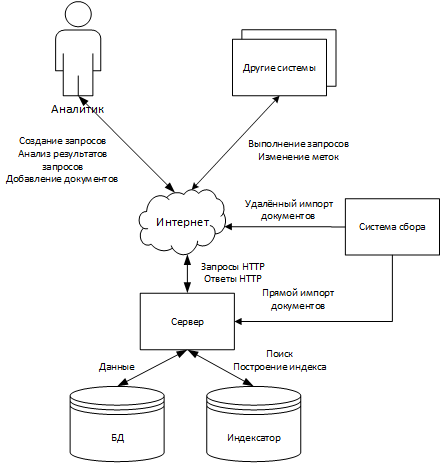
\includegraphics{design/domain}
\caption{Схема предметной области.}
\label{figure:domain}
\end{figure}

\clearpage
\subsubsection{Сущности предметной области}

В процессе анализа предметной области выделены основные сущности:
\begin{itemize}
\item Запрос;
\item Прогноз;
\item Регион;
\item Страна;
\item Провинция;
\item Сценарий;
\item Аналитическая записка;
\end{itemize}

Дополнительные сущности, наличие которых следует из основных:
\begin{itemize}
\item Полином -- параметры полинома в полиноминальной регрессии
\item Скользящее среднее -- параметры для алгоритма скользящего среднего
\item Измерение прогноза -- сохранённый результат выполнения запроса прогноза по дням;
\item Популяция прогноза -- коллекция формул для прогноза;
\item Приспособленность -- история лучших и средних значений функции приспособленности по поколениям для популяции;
\item Веса -- веса для итоговой оценки методом средневзвешенной суммы
\end{itemize}

Выявлены следующие акторы:
\begin{itemize}
\item Пользователь -- основной пользователь подсистемы
\item Эксперт -- создаёт/редактирует запросы, редактирует контура стран/провинций
\end{itemize}

Выявлены следующие источники данных:
\begin{itemize}
\item ИПС -- предоставляет API доступа и редактирования к актуальной базе новостей
\item Эксперт -- создаёт/редактирует запросы, редактирует контура стран/провинций
\end{itemize}

\subsubsection{Описание бизнес-процесса}
Автоматизации подлежат следующие процессы системы:
\begin{itemize}
\item Разметка документов базы геометками;
\item Прогнозирование новостных потоков;
\item Построение сценария развития ситуации;
\item Создание аналитической записки;
\end{itemize}

Новости агрегируются в ИПС. Модуль геотегирования размечает новости согласно сохранённым в Волхв-ГЕО запросам. Размеченные новости используются для прогнозирования ситуации и отображения на карте.

Схема бизнес-процесса представлена в графической части на листе <<Бизнес-процесс подсистемы>>

\includepdf[pages=5]{A1.pdf}

\subsubsection{Выбор и обоснование критериев качества}

Для данной подсистемы можно выделить следующие критерии качества:
\begin{itemize}
\item Пользовательский интерфейс;
\item Геопривязка;
\item Автоматизация;
\item Интеграция;
\item Прогноз;
\item Сценарии.
\end{itemize}

\paragraph{Пользовательский интерфейс.}
Означает простоту и понятность работы с системой. Оценивается:
\begin{itemize}
\item Структура сайта;
\item Степень интуитивной понятности меню;
\end{itemize}

\paragraph{Геопривязка.}
Означает точность привязки события на карте. Оценивается:
\begin{itemize}
\item Информативность геопривязки;
\item Отклонение геометки от реального места событий.
\end{itemize}

\paragraph{Автоматизация.}
Оценивает количество функций выполняемых в автоматическом режиме.

\clearpage
\paragraph{Интеграция.} 
Обозначает возможность и удобство интеграции подсистемы с другими системами. Оценивается:
\begin{itemize}
\item Наличие интеграционного интерфейса;
\item Удобность этого интерфейса для разработчиков;
\item Полнота интерфейса (полная реализация всех возможностей системы в интерфейсе).
\end{itemize}

\paragraph{Прогноз.} 
Обозначает наличие прогнозирующего функционала и качество прогноза. Оценивается:
\begin{itemize}
\item Возможность автоматизированного прогнозирования;
\item Качество прогноза;
\end{itemize}

\paragraph{Сценарии.} 
Обозначает наличие инструментария для создания и редактирования сценариев и аналитических заметок. Оценивается:
\begin{itemize}
\item Наличие инструментария;
\item Качество инструментов;
\end{itemize}

Присвоим критериям качества следующие весовые коэффициент, которые отображены в таблице~\ref{table:qualityWeights}.

\begin{table}[h!]
\centering
\caption{Критерии качества и их весовые коэффициенты}
\label{table:qualityWeights}
\begin{tabular}{L{10cm}|C{3cm}}
\multicolumn{1}{C{10cm}|}{Критерий} & 
\multicolumn{1}{C{3cm}}{$\alpha$} \\
\hline\hline

Пользовательский интерфейс & 0.1 \\
Геопривязка & 0.2 \\
Автоматизация & 0.25 \\
Интеграция & 0.15 \\
Прогноз & 0.2 \\
Сценарии & 0.1 \\

\end{tabular}
\end{table}

Выполнено следующее условие:
\begin{equation}
\sum \alpha_i = 0.1 + 0.2 + 0.25 + 0.15 + 0.2 + 0.1 = 1
\end{equation}

\subsubsection{Перечень задач, подлежащих решению в процессе разработки}

В процессе разработки необходимо решить следующие задачи:
\begin{itemize}
\item исследование и анализ предметной области;
\item анализ и определение критериев качества;
\item определение функциональных требований разрабатываемой системы;
\item разработка структуры модулей системы, с выделением функциональности для каждого модуля;
\item проектирование базы данных: инфологическая, даталогическая модели;
\item проектирование эволюционного алгоритма прогнозирования;
\item рассмотрение и обоснование архитектуры системы;
\item выбор программных библиотек для реализации модулей;
\item разработка интерфейса взаимодействия пользователя с программой;
\item реализация графа диалога;
\item написание и отладка программного кода модулей системы;
\item разработка технической документации.
\end{itemize}

\clearpage
\subsubsection{Анализ аналогов и прототипов}

Для расчета нормированного значения j-го варианта по i-ому критерию необходимо
воспользоваться формулой~\ref{equation:criteria}.

\begin{equation}
\label{equation:criteria}
K_{ij} = \frac{x_{ij} - x_i^-}{x_i^+ - x_i^-}
\end{equation}
\begin{ESKDexplanation}
\item[где ] $x_{ij}$ - натуральное значение;
\item       $x_i^+$ - максимальное значение;
\item       $x_i^-$ - минимальное значение.
\end{ESKDexplanation}

Для расчета интегрального показателя воспользуемся формулой~\ref{equation:criteriaTotal}.

\begin{equation}
\label{equation:criteriaTotal}
K = \sum_{i=1}^m \alpha_i K_{ij}
\end{equation}
\begin{ESKDexplanation}
\item[где ] $m$ - количество критериев.
\end{ESKDexplanation}

Оценка по критериям производится путём присуждения баллов в соответствии со шкалой, представленной в таблице~\ref{table:criteria}.

\begin{table}[h!]
\centering
\caption{Критерии качества и их весовые коэффициенты}
\label{table:criteria}
\begin{tabular}{L{4cm}|C{2cm}|C{2cm}|C{2cm}|C{2cm}|C{2cm}}
\multicolumn{1}{C{4cm}|}{Качественный показатель} & 
\multicolumn{1}{C{2cm}|}{Отлично} & 
\multicolumn{1}{C{2cm}|}{Хорошо} & 
\multicolumn{1}{C{2cm}|}{Удовлетворительно} & 
\multicolumn{1}{C{2cm}|}{Плохо} & 
\multicolumn{1}{C{2cm} }{Неудовлетворительно} \\
\hline\hline

Количественный показатель & 5 & 4 & 3 & 2 & 1 \\
$K_{ij}$ & 1 & 0.75 & 0.5 & 0.25 & 0 \\

\end{tabular}
\end{table}

Прямых и полных аналогов проектируемой подсистемы нет, но есть проекты, реализующие части функционала:
\begin{itemize}
\item http://liveuamap.com/
\item http://militarymaps.info/
\end{itemize}

\clearpage
Эти аналоги имеют ряд принципиальных недостатков и не могут отвечать всем
требованиям.

Недостатками аналога «http://liveuamap.com/» являются:
\begin{itemize}
\item отсутствие системы прогнозирования;
\item отсутствие инструментария для создания сценария и аналитических записок;
\item узкий набор отслеживаемых тем;
\item невозможность добавить новость.
\end{itemize}

Недостатками аналога «http://militarymaps.info/» являются:
\begin{itemize}
\item отсутствие системы прогнозирования;
\item отсутствие инструментария для создания сценария и аналитических записок;
\item узкий набор отслеживаемых тем;
\item перегруженный интерфейс.
\end{itemize}

Сравним аналоги и прототипы без учета весовых коэффициентов, результаты сведены в таблицу~\ref{table:analogs1}.

\begin{table}[h!]
\centering
\caption{Сравнение аналогов и прототипов без учета весовых коэффициентов}
\label{table:analogs1}
\begin{tabular}{L{5cm}|C{3cm}|C{3cm}|C{3cm}}
\multicolumn{1}{C{5cm}|}{Критерий} & 
\multicolumn{1}{C{3cm}|}{liveuamap} & 
\multicolumn{1}{C{3cm}|}{militarymaps} & 
\multicolumn{1}{C{3cm}}{Волхв-ГЕО} \\
\hline\hline

Пользовательский интерфейс & 4 & 2 & 4 \\ \hline
Геопривязка & 4 & 4 & 3 \\ \hline
Автоматизация & 2 & 2 & 4 \\ \hline
Интеграция & 1 & 2 & 3 \\ \hline
Прогноз & 2 & 1 & 3 \\ \hline
Сценарии & 2 & 3 & 4 \\ \hline
\hline
Итого & 15 & 14 & 21 \\

\end{tabular}
\end{table}

Сравним аналоги и прототипы с учетом весовых коэффициентов, результаты сведены в таблицу~\ref{table:analogs2}.

\clearpage
\begin{table}[h!]
\centering
\caption{Сравнение аналогов и прототипов с учётом весовых коэффициентов}
\label{table:analogs2}
\begin{tabular}{L{5cm}|C{1cm}|C{3cm}|C{3cm}|C{3cm}}
\multicolumn{1}{C{5cm}|}{Критерий} & 
\multicolumn{1}{C{1cm}|}{$\alpha$} & 
\multicolumn{1}{C{3cm}|}{liveuamap} & 
\multicolumn{1}{C{3cm}|}{militarymaps} & 
\multicolumn{1}{C{3cm}}{Волхв-ГЕО} \\
\hline\hline

Пользовательский интерфейс & 0.1 & 0.75 & 0.5 & 0.75 \\ \hline
Геопривязка & 0.2 & 0.75 & 0.75 & 0.25 \\ \hline
Автоматизация & 0.25 & 0.5 & 0.5 & 0.75 \\ \hline
Интеграция & 0.15 & 0.0 & 0.5 & 0.25 \\ \hline
Прогноз & 0.2 & 0.5 & 0.0 & 0.25 \\ \hline
Сценарии & 0.1 & 0.5 & 0.25 & 0.75 \\ \hline
\hline
Итого & 1 & 0.3625 & 0.9375 & 1.25 \\

\end{tabular}
\end{table}

Таким образом, подсистема «Волхв-ГЕО» является лучшей среди аналогов и
оправдывает свое создание.
\subsection{Разработка интерфейса взаимодействия}

Интерфейс взаимодействия с пользователем основан на HTML с применением
технологии Ajax с целью повысить удобство использования. Такой выбор был сделан на
основе специфики разрабатываемой системы и анализа требований к веб-приложению.
Необходимым условием взаимодействия пользователя с системой является наличие
современного веб-браузера, поддерживающего язык JavaScript и спецификацию HTML 4.0
(Mozilla Firefox 4.0, Google Chrome 10 и т.п.).

\subsubsection{Разработка графа диалога}

Граф диалога проектируемой подсистемы:

\begin{figure}[!h]
\centering
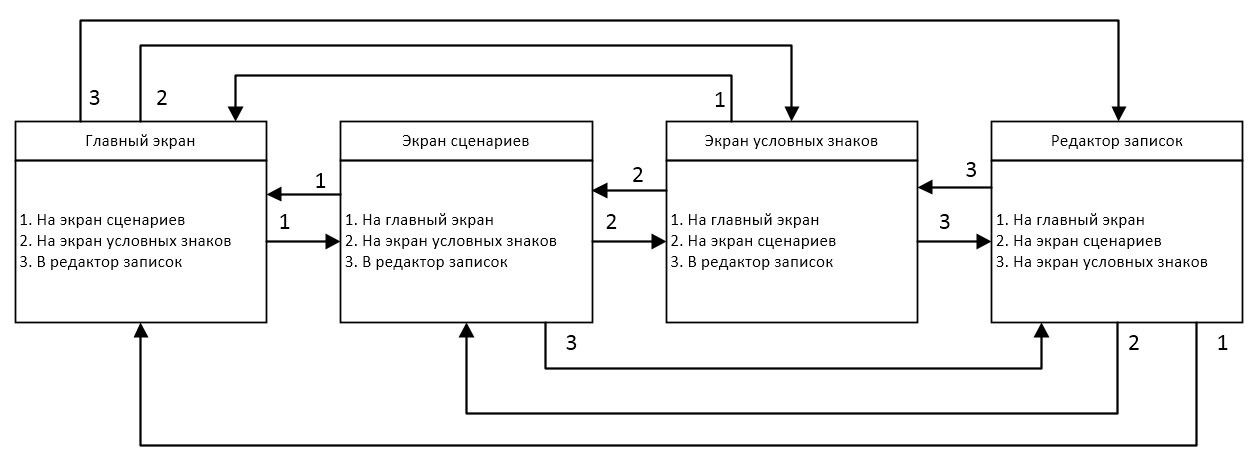
\includegraphics[width=\textwidth]{technology/graph}
\caption{Граф диалога.}
\label{figure:dialogGraph}
\end{figure}

\subsubsection{Разработка экранных форм}

Для разработки экранных форм выбрана библиотека Bootstrap, обеспечивающая эргономический и единообразный интерфейс, что соответствует требованиям проекта.

\subsection{Описание экранных форм}

\begin{figure}[!h]
\centering
\includegraphics[width=\textwidth]{technology/gui/1}
\caption{Начальный экран.}
\label{figure:gui1}
\end{figure}

Слева представлено основное меню клиентского приложения. Карта продолжает отображаться при выборе любого из пунктов меню.

\clearpage
\begin{figure}[!h]
\centering
\includegraphics{technology/gui/2}
\caption{Виды условных знаков.}
\label{figure:gui2}
\end{figure}

Приложение поддерживает три типа условных знаков:

\begin{itemize}
\item События -- для отметки точечных событий, объектов
\item Области -- для отметки распределённых по площади объетов: позиций сторон, площадей затопления, возгорания итп.
\item Стрелки -- для отметки передвижения, направления распространения объектов 
\end{itemize}

\clearpage
\begin{figure}[!h]
\centering
\includegraphics[width=\textwidth]{technology/gui/3}
\caption{Интенсивность новостей по странам.}
\label{figure:gui3}
\end{figure}

В этом режиме отображения с помощью тепловой карты отображается скорость поступления новостей по странам.

\begin{figure}[!h]
\centering
\includegraphics[width=\textwidth]{technology/gui/4}
\caption{Пример отображения прогноза.}
\label{figure:gui4}
\end{figure}

Пример отображения прогноза: при клике левой кнопкой мыши на провинцию, появляется всплывающее окно с пятью наиболее активными темами данной провинции и рядом с ними даётся прогноз изменения активности -- количества новостей за период времени, на прогнозируемый период.

\begin{figure}[!h]
\centering
\includegraphics[width=\textwidth]{technology/gui/5}
\caption{Пример сценария.}
\label{figure:gui5}
\end{figure}

Сценарий по замыслу представляет собой набор элементов карты.

\begin{figure}[!h]
\centering
\includegraphics[width=\textwidth]{technology/gui/6}
\caption{Редактор аналитической записки.}
\label{figure:gui6}
\end{figure}

Аналитическая записка является сопровождением к сценарию и составляется в разметке markdown.

%===========================================================================
% Исследовательская часть
\section{Исследовательская часть}

\subsection{Эволюционный алгоритм}

Теоретическое обоснование генетических алгоритмов приводится в работе Дж. Холланда [1]. 
Ключевой является теорема схем, доказывающая эффективность генетического алгоритма. Теорема схем показывает происходящее при смене поколений экспоненциальное распространение хорошо приспособленных схем.

Эта теорема, вкупе с решением задачи многорукого бандита [3] показывает, что генетические алгоритмы являются наиболее быстрым методом поиска в пространствах с неизвестными свойствами.

Теорема схем формулируется для представления генома в виде битовых строк фиксированной длины.

Для обоснованности применения данной теоремы к деревьям вычисления достаточно ввести ограничение на максимальную глубину дерева, добавить некоторый виртуальный оператор-заглушку и добавив виртуальные параметры привести все операторы к одной арности. В таком случае все деревья будут иметь одинаковую структуру и количество узлов. Тогда их можно взаимно отобразить в бинарные строки фиксированной длины и структуры. Таким образом, теорема схем применима и в случае деревьев вычислений.

\clearpage
\subsubsection{Алгоритм скрещивания} \label{sssec:crossover}
В разрабатываемом модуле эволюционирующей структурой является дерево вычислений. Это влечёт за собой отличия от классического генетического алгоритма, применяемого к битовым строкам или массивам.

Хотя формулу можно представить в виде строки, скрещивание напрямую двух строк одноточечным или многоточеченым скрещиванием является крайне неэффективным методом, так как при этом нарушается вложенность скобок, разрываются операция и её аргументы и подавляющее большинство формул-потомков являются некорректными и невычислимыми.

\begin{figure}[!h]
\centering
\includegraphics[scale=0.7]{research/pics/1.png}
\caption{Иллюстрация многоточечного скрещивания массива..}
\label{figure:arrayCrossover}
\end{figure}


По этой причине была выбрана схема скрещивания поддеревьями. Формула представляется в виде дерева вычислений. Для скрещивания в каждом дереве выбирается узел. Каждый выбранный узел – корень некоторого поддерева. Скрещивающиеся деревья обмениваются соответствующими поддеревьями, образуя пару потомков.

Пример: скрещивание деревьев, описывающих формулы 

  sin(X0^2)+X1*2.3

  sqrt(X0/3.14)*(X1+X0^2)

с корнями поддеревьев в +, \^{} (возведение в степень) соответственно, даёт:

  sin(X0 + 1) + X1 * 2.3

  sqrt(X0 / 3.14) * (X1 + X0 + 1)

\clearpage
\begin{figure}[!h]
\centering
\includegraphics[scale=0.5]{research/pics/2.png}

=

\includegraphics[scale=0.5]{research/pics/3.png}
\label{figure:crossover}
\caption{Пример скрещивания деревьев}
\end{figure}

У такого метода скрещивания есть одна особенность. Если у первого родителя можно выбирать абсолютно любой узел, то для второго родителя такой подход может вести к превышению максимально допустимой глубины. Проиллюстрируем примером:

Возьмём деревья из предыдущего примера и установим максимально допустимую глубину дерева = 4. Оба родителя выполняют это условие. 

Будем выбирать случайные узлы у обоих родителей. Может сложиться такая ситуация:

\clearpage
\begin{figure}[!h]
\centering
\includegraphics[scale=0.5]{research/pics/4.png}

=

\includegraphics[scale=0.5]{research/pics/5.png}
\label{figure:crossoverOverflow}
\end{figure}

Как мы видим, несмотря на то что после скрещивания получились корректные с математической точки зрения формулы, первое дерево превысило максимально допустимую глубину.

Происходит это из за серьёзного отличия от скрещивания массивов. В случае массивов  оба родителя имеют одинаковую структуру и длину. Поэтому точка, выбранная на одном массиве, имеется и на другом, и, обменяв эти точки, мы получаем заведомо подоходящих по структуре и длине потомков. 

Деревья-родители же имеют различную структуру и размеры. Поэтому такой подход в принципе не возможен. 

Чтобы избежать разрастания в глубину, для второго дерева выбор узлов для обмена должен осуществляться только среди таких узлов, при выборе которых не нарушится ограничение по глубине -- <<хороших>> узлов.

\subsubsection{Поиск «хороших» узлов}

Для рассуждений в данном случае деревья удобнее представлять как линейные структуры. Общее правило от этого не изменится.

Точки 2 и 4 обозначают глубину первого и второго дерева соответственно.

Точки 1 и 3 обозначают выбранные для скрещивания 

d1, d2 -- глубина точек 1 и 3.

h1, h2 -- высота точек 1 и 3.

\begin{figure}[!h]
\centering
\includegraphics[scale=0.7]{research/pics/6.png}
\label{figure:arrayGoodNodes1}
\end{figure}

Условие, что глубины деревьев-родителей меньше максимальной:

\begin{equation}
\label{equation:goodNodesEq1}
\begin{cases} d1 + h1 \leq Max_{depth} \\ d2 + h2 \leq Max_{depth} \end{cases}
\end{equation}

После скрещивания получим новые деревья. 

\begin{figure}[!h]
\centering
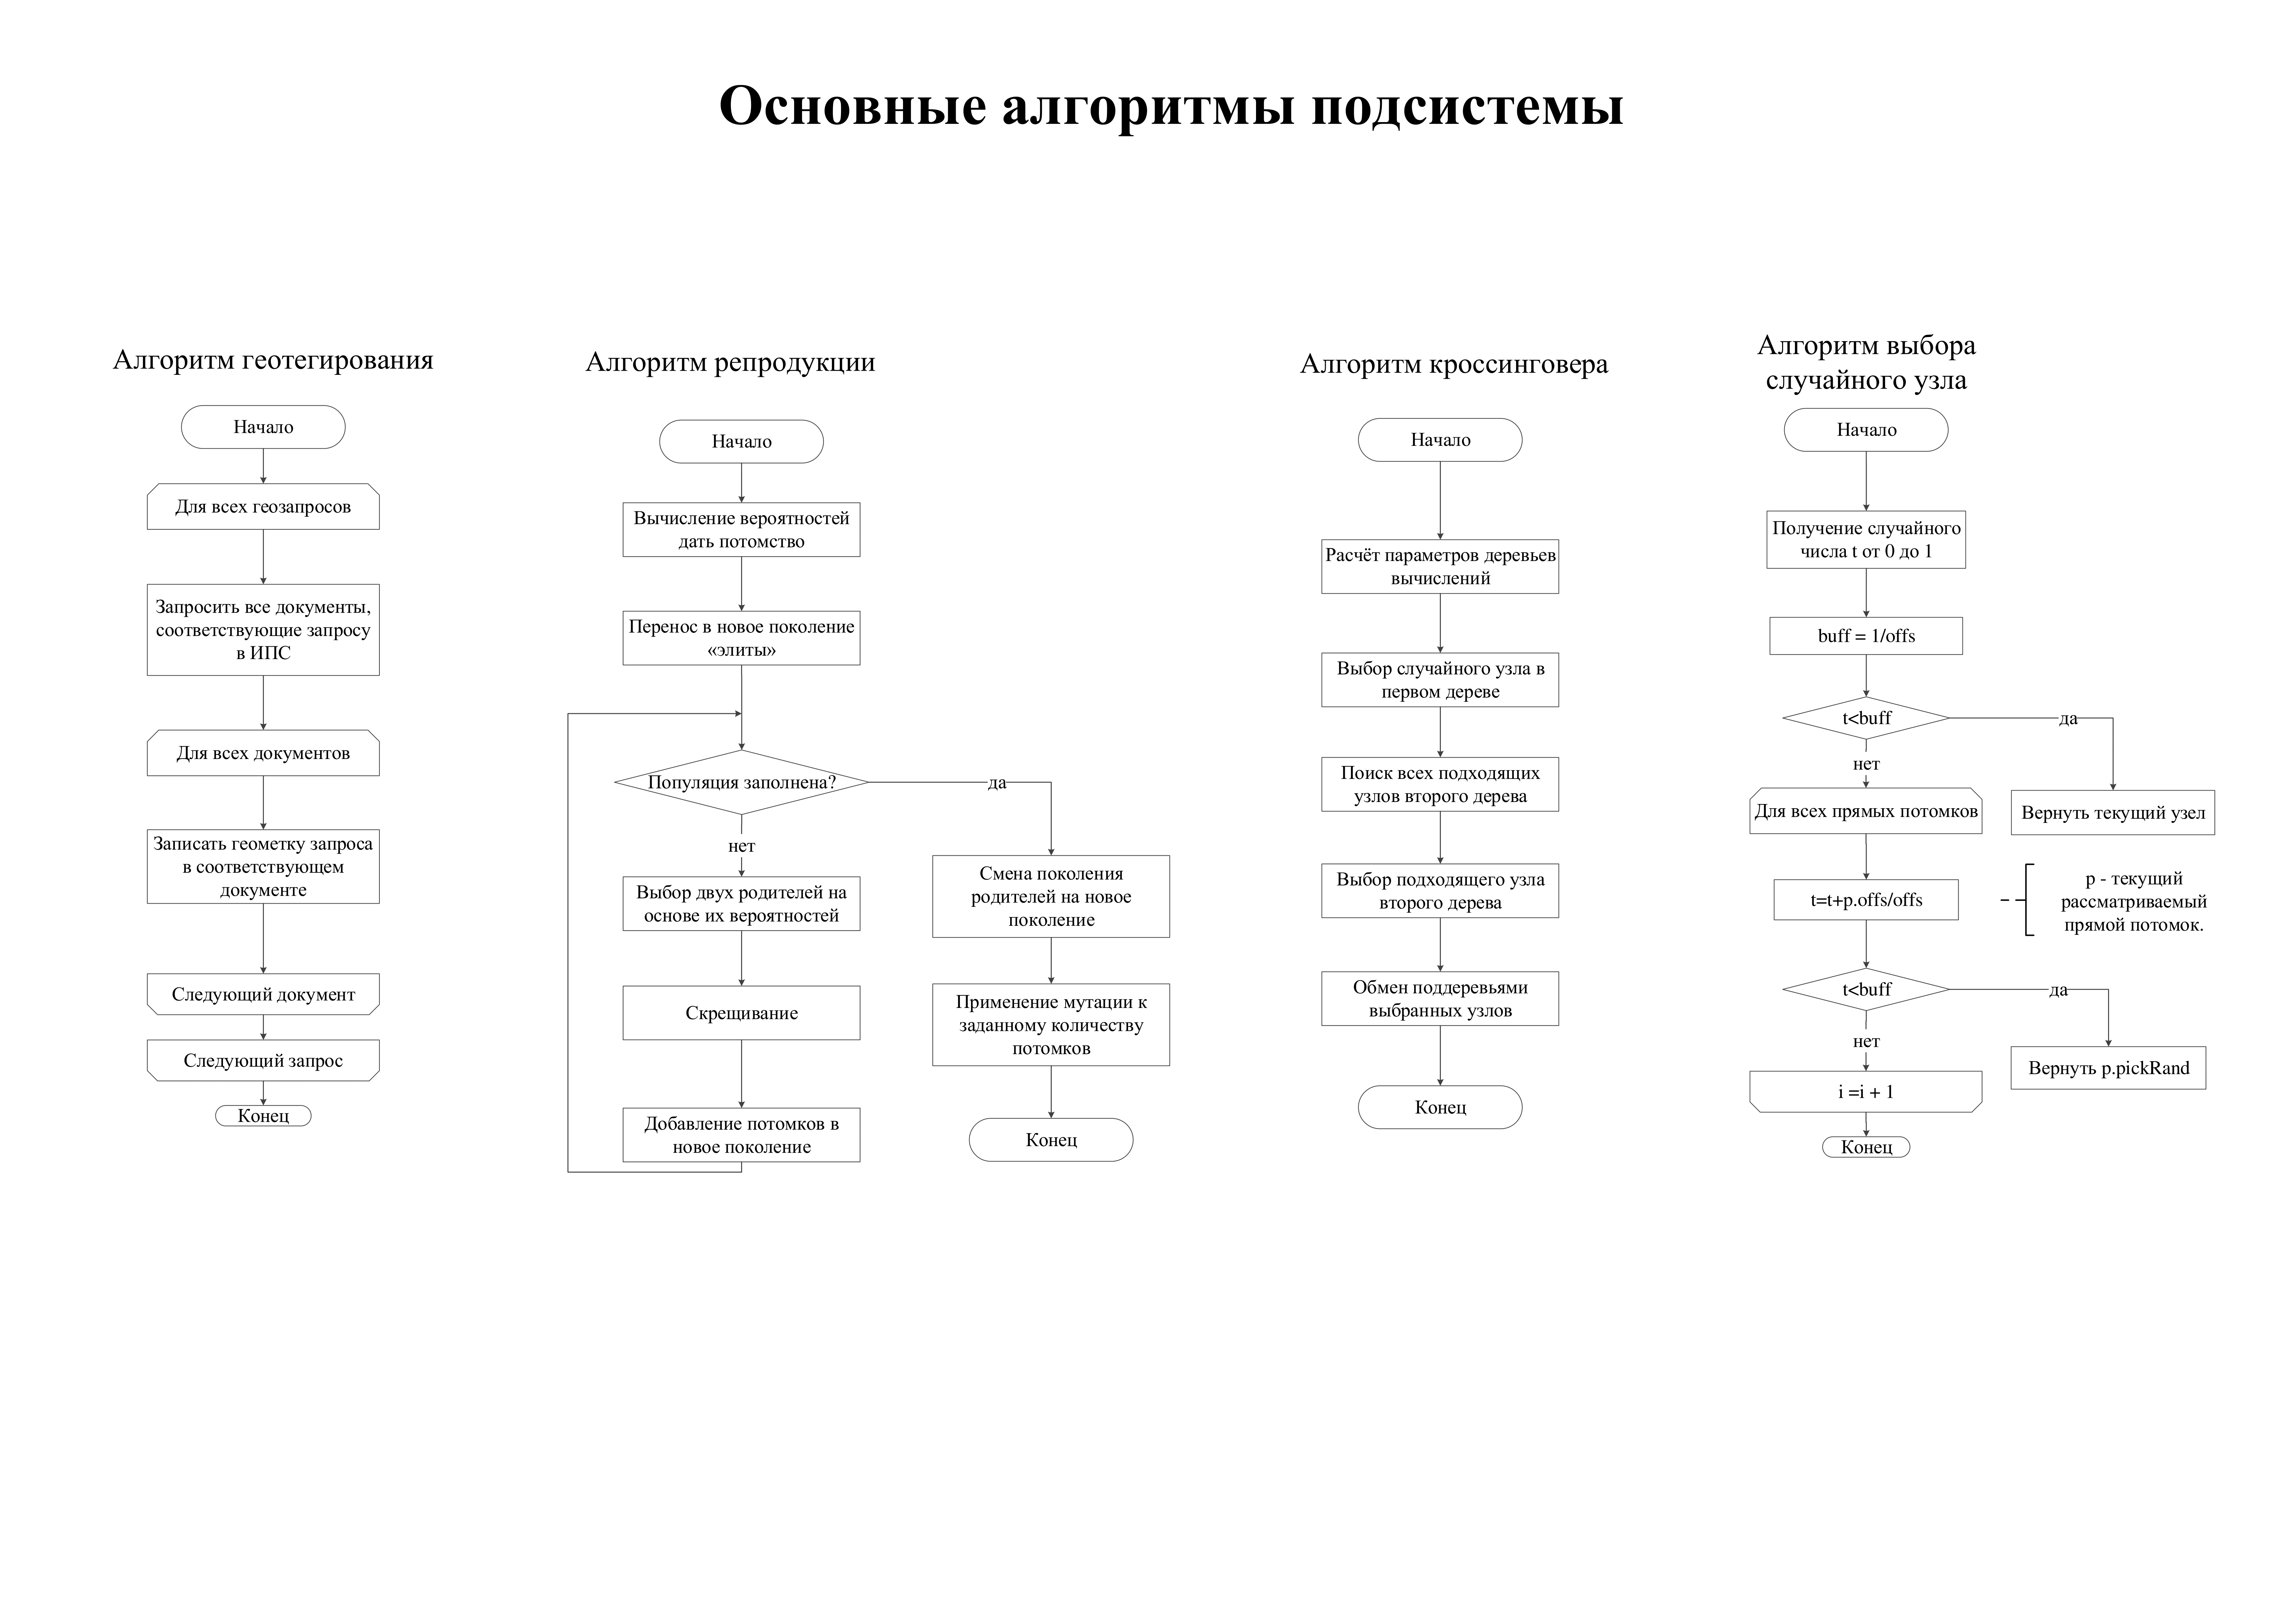
\includegraphics[scale=0.7]{research/pics/7.png}
\label{figure:arrayGoodNodes2}
\end{figure}

Запишем условие по глубине:

\begin{equation}
\label{equation:goodNodesEq2}
\begin{cases}d2 + h1 \leq Max_{depth} \\  d1 + h2 \leq Max_{depth} \end{cases}
\end{equation}

\clearpage
Отсюда получим условие для подходящих узлов:

\begin{equation}
\label{equation:goodNodesEq3}
\begin{cases} d2 \leq Max_{depth} - h1 \\ h2 \leq Max_{depth} - d1  \end{cases}
\end{equation}

Все узлы, удовлетворяющие условию \ref{equation:goodNodesEq3}, являются «хорошими». Выбор узла среди них осуществляется случайным образом.

\subsubsection{Алгоритм мутации}

Мутация -- одна из ключевых операций эволюционного алгоритма.

В подсистеме применяется следующий алгоритм мутации:
\begin{enumerate}
\item Случайным образом выбирается узел дерева. Вероятность выбора для всех узлов дерева одинакова.
\item Выбранный узел, вместе с его поддеревом, заменяется на новое поддерево, генерируемое по общим правилам, с учётом условия на максимальную глубину. 
\end{enumerate}

\clearpage
\begin{figure}[!h]
\centering
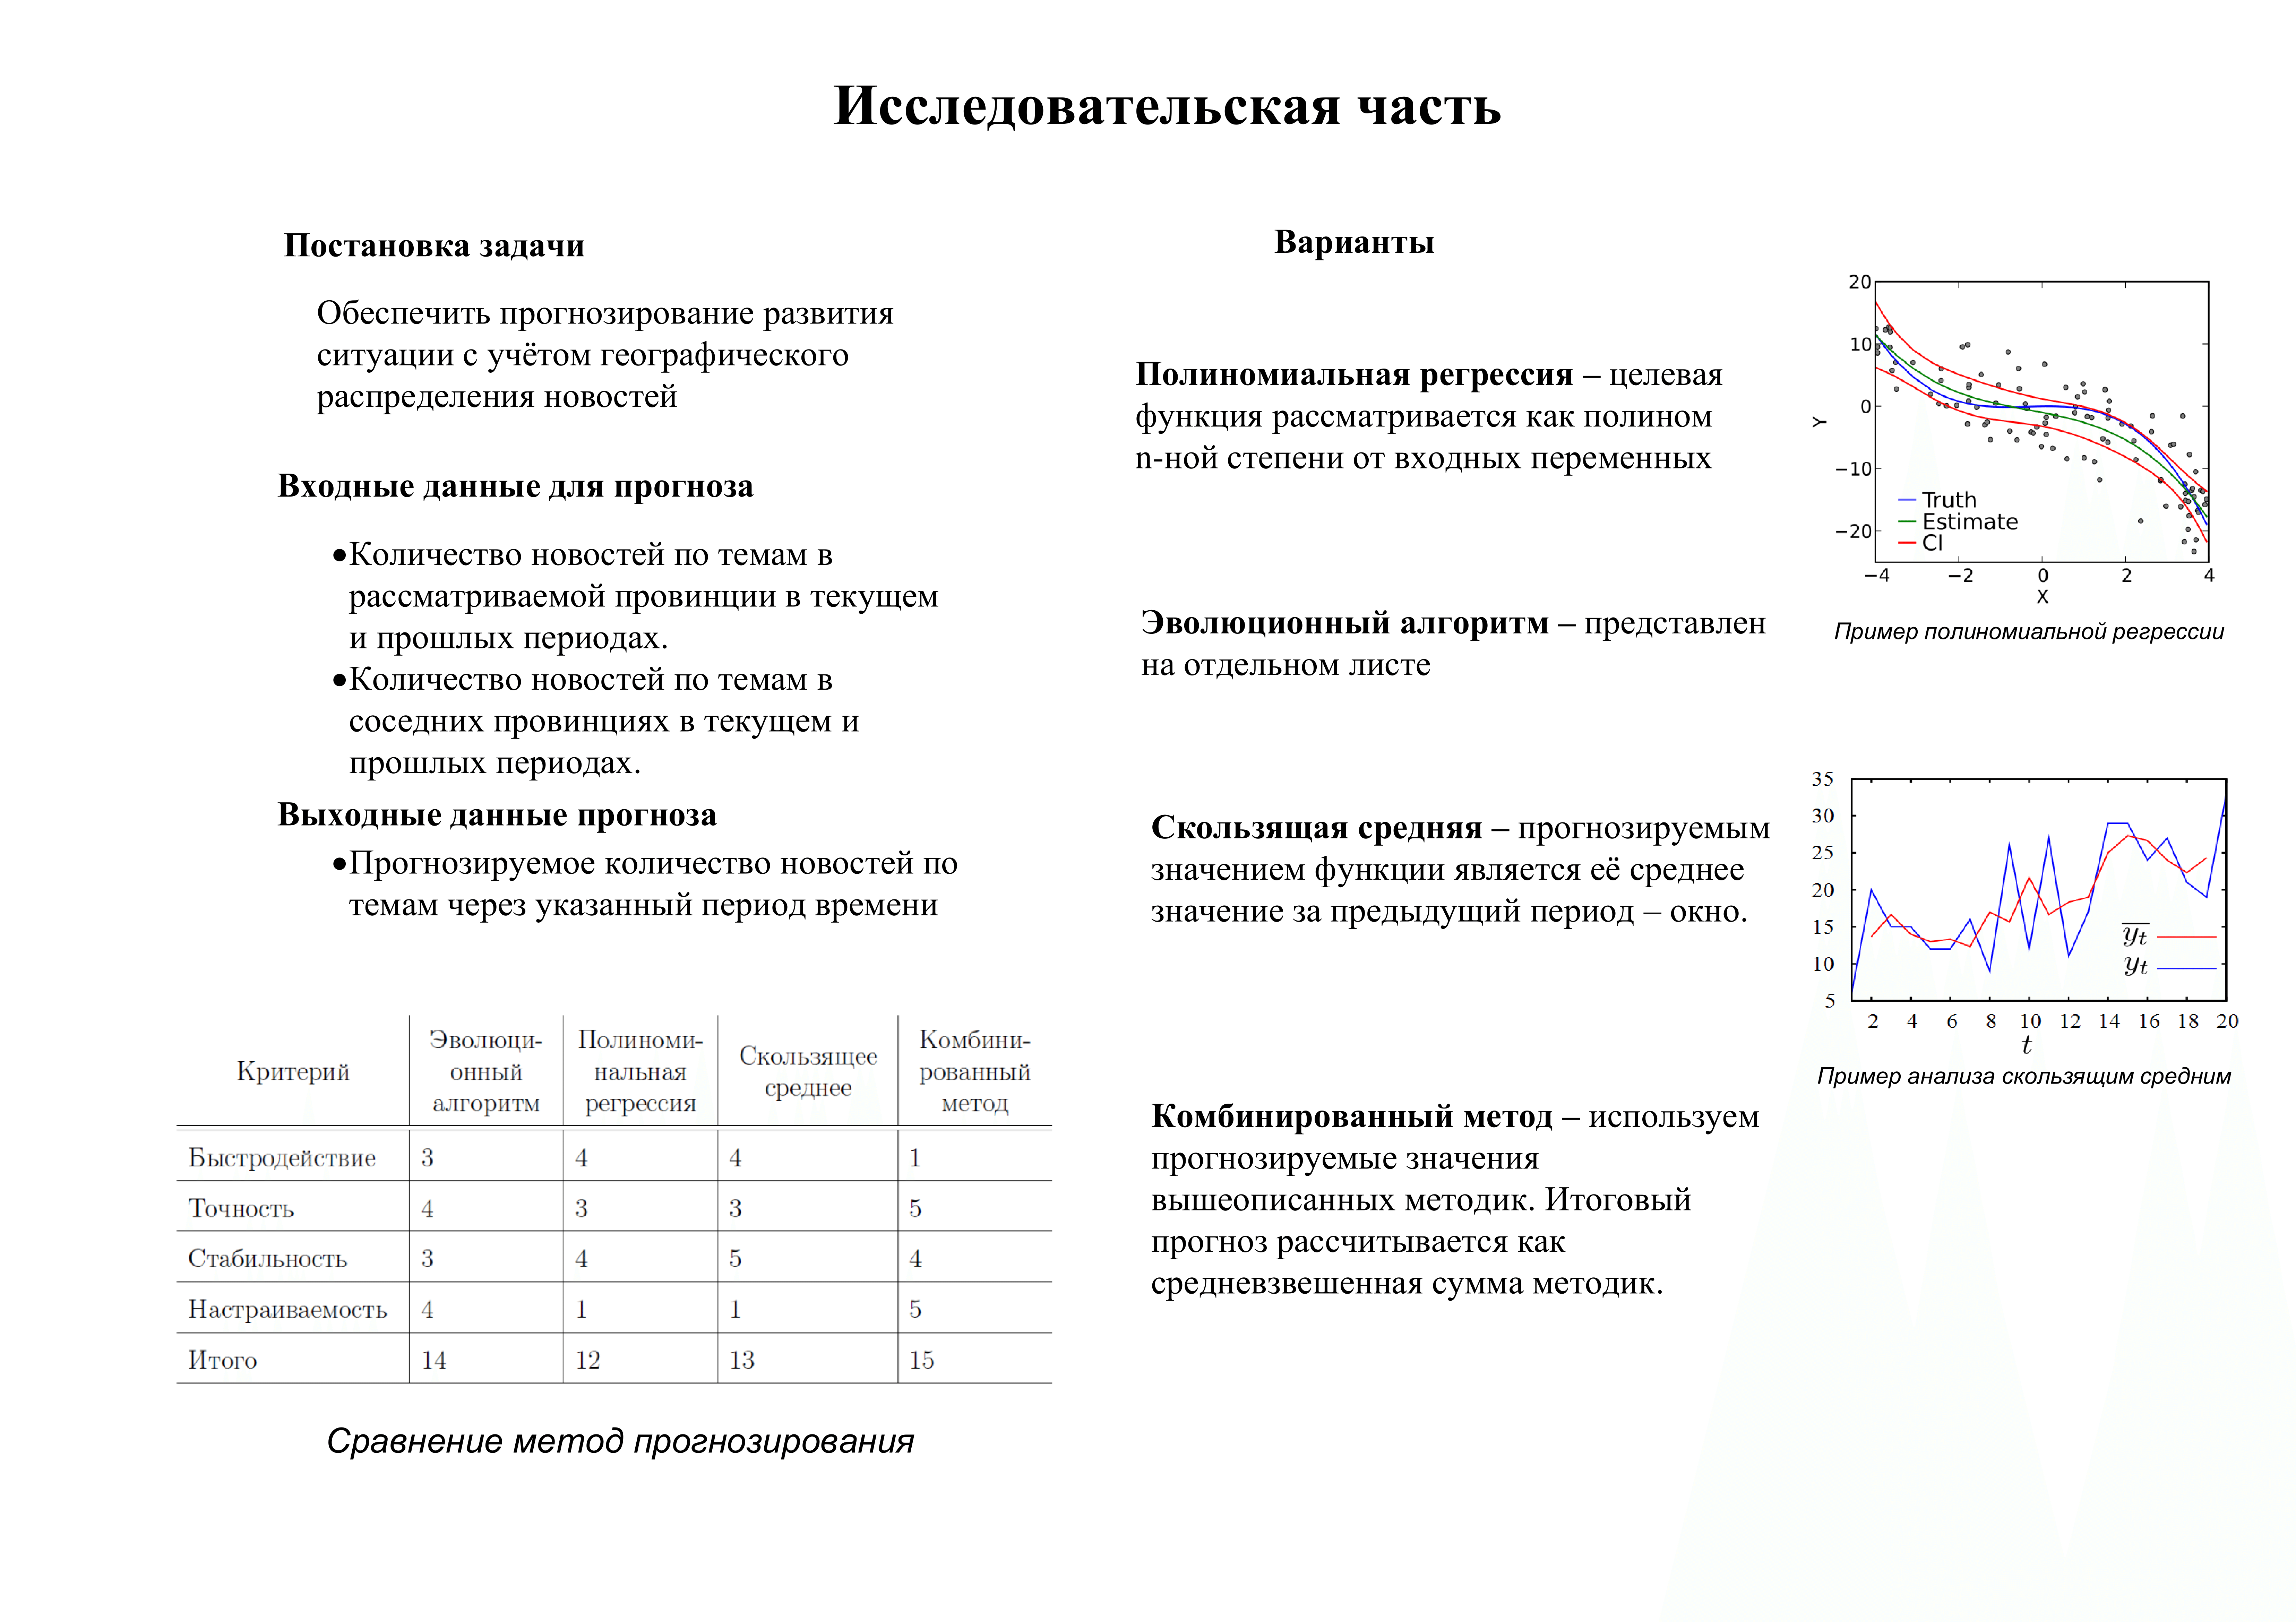
\includegraphics[scale=0.7]{research/pics/8.png}

=>

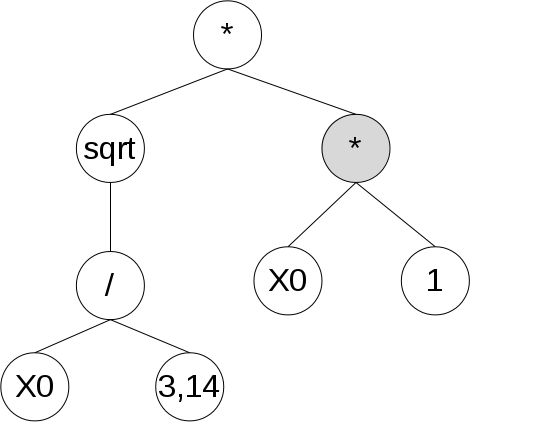
\includegraphics[scale=0.7]{research/pics/9.png}
\label{figure:mutation}
\caption{Пример мутации}
\end{figure}

Для осуществления этого, необходимо реализовать равномерное распределение вероятностей для узлов графа. Что является интересной задачей, учитывая, что алгоритм выбора узлов должен быть рекурсивным и что дерево – структура данных без случайного доступа. 


\clearpage
\subsubsection{Равномерное распределение на узлах дерева}

Выбор с одинаковой вероятностью среди узлов дерева реализовывается таким образом:

В каждом узле хранится числова характеристика offs, которая равна количеству всех потомков узла + 1 (сам узел). Количество потомков расчитывается рекурсивно:

\begin{equation}
\label{equation:goodNodesEq3}
offs(ind) = \begin{cases} 1, & \mbox{для листьев дерева} \\ 1 + \sum_i(offs(child_i)), & \mbox{для прочих вершин} \end{cases}
\end{equation}

Выбор осуществляется с корневого узла дерева. Алгоритм выбора приведён далее.

\clearpage
\begin{figure}[!h]
\centering
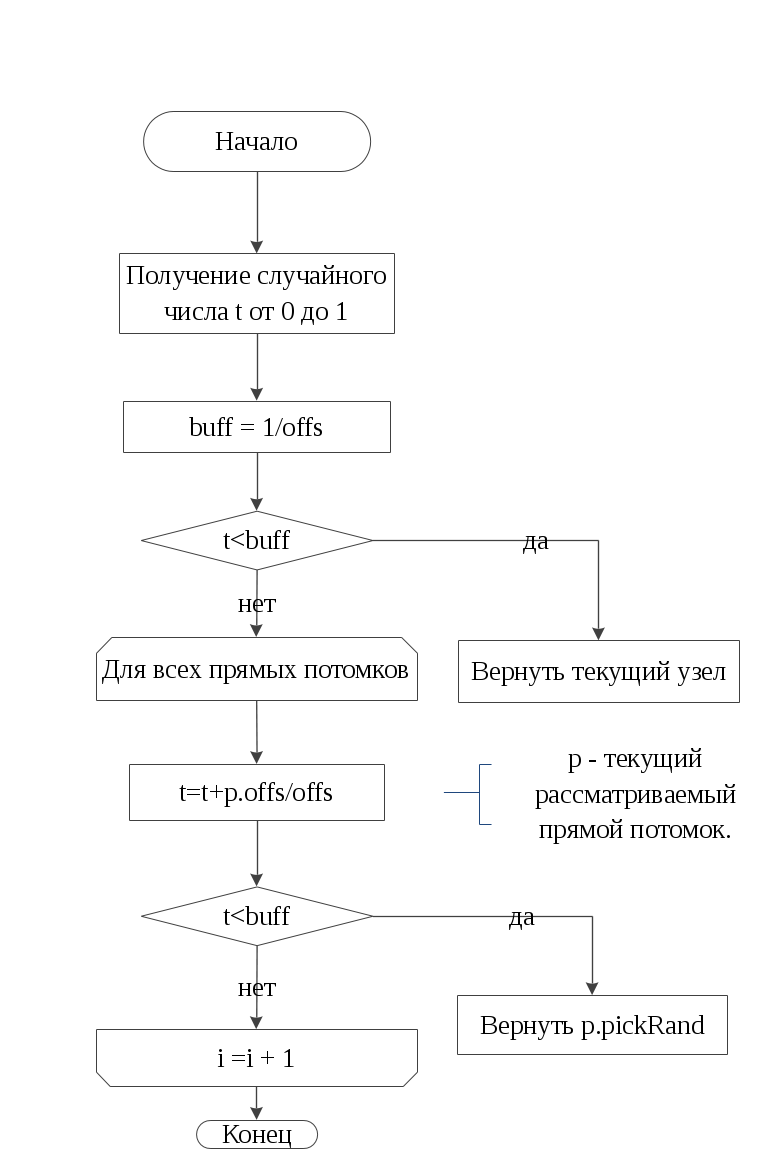
\includegraphics[scale=0.7]{research/pics/12.png}
\label{figure:randomPick}
\end{figure}

\clearpage
Проверим алгоритм:


\begin{figure}[!h]
\centering
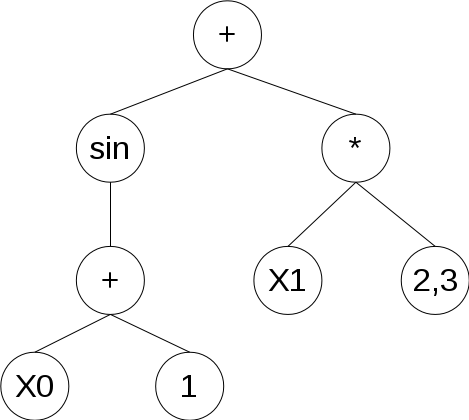
\includegraphics[scale=0.4]{research/pics/10.png}
\caption{Дерево}
\label{figure:offsTree1}
\end{figure}
\begin{figure}[!h]
\centering
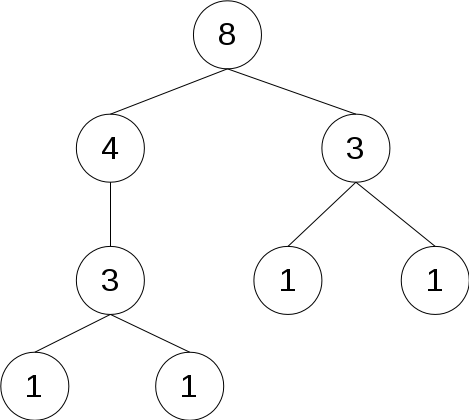
\includegraphics[scale=0.4]{research/pics/11.png}
\caption{Дерево offs}
\label{figure:offsTree2}
\end{figure}

Для дерева \ref{figure:offsTree1} вероятность выбрать любой узел должна равняться $\frac{1}{8}$.

\renewcommand{\arraystretch}{1.5}

\begin{table}[h!]
\centering
\caption{Вероятность выбора узла}
\begin{tabular}{L{4cm}|L{8cm}}
\multicolumn{1}{C{4cm}|}{Узел} & 
\multicolumn{1}{C{8cm}}{Вероятность} \\
\hline\hline

Корень & $\frac{1}{8}$ \\ \hline
sin & $\frac{4}{8} \cdot \frac{1}{4} = \frac{1}{8}$ \\ \hline
+ & $\frac{4}{8} \cdot \frac{3}{4} \cdot \frac{1}{3} = \frac{1}{8}$ \\ \hline
X0 & $\frac{4}{8} \cdot \frac{3}{4} \cdot \frac{2}{3} \cdot \frac{1}{2} = \frac{1}{8}$ \\ \hline
1 & $\frac{4}{8} \cdot \frac{3}{4} \cdot \frac{2}{3} \cdot \frac{1}{2} = \frac{1}{8}$ \\ \hline
* & $\frac{3}{8} \cdot \frac{1}{3} = \frac{1}{8}$ \\ \hline
X1 & $\frac{3}{8} \cdot \frac{2}{3} \cdot \frac{1}{2} = \frac{1}{8}$ \\ \hline
2.3 & $\frac{3}{8} \cdot \frac{2}{3} \cdot \frac{1}{2} = \frac{1}{8}$ \\ \hline

\end{tabular}
\end{table}

Как видим, для всех узлов вероятность выбора = $\frac{1}{8}$.

Так же вполне очевидно, что это правило работает и в общем случае.

\subsubsection{Выбор стратегии скрещивания}

Скрещивание двух деревьев описано в пункте \ref{sssec:crossover}. Встаёт вопрос выбора конкретных родителей из множества всех индивидов.

Возможны различные способы выбора, основанные на идее, что индивид с большим значением приспособленности, должен иметь больший шанс дать потомство.

Некоторые из способов:
\begin{itemize}
\item Пропорциональный
\item Состязание
\end{itemize}

Опишем каждый из них в отдельности.

\paragraph{Пропорциональный} \label{par:prop}

Для каждого индивида рассчитывается вероятность оставить потомство.

\begin{equation}
\label{equation:propF1}
p_i = \frac{f_i}{\sum_{j=1}^N(f_j)}
\end{equation}
\begin{ESKDexplanation}
\item[где ] $f_i$ -- приспособленность i-го индивида,
\item $N$ -- количество индивидов
\end{ESKDexplanation}

Выполняется условие:

\begin{equation}
\label{equation:propF1}
\sum_{i=1}^N(p_i) = 1
\end{equation}

Выбираются 2 родителя согласно описанному распределению вероятностей и дают 2 потомка, которые добавляются в новое поколение. 

Эти действия повторяются, пока новое поколение не будет заполнено.

\paragraph{Состязание}

Моделируется такое явление живой природы, как бои за право спаривания.

Выбираются два случайных индивида, и проводится «состязание». Индивид с наибольшим значением фитнеса считается победителем.

Выбирается вторая пара и определяется второй победитель.

Победители образуют пару и дают потомство.

\paragraph{Выбор стратегии}

Критерии:

\begin{itemize}
\item Вычислительная сложность
\item Затраты памяти
\item Скорость схождения
\end{itemize}

Сравнение проведём по методу Борда

\begin{table}[h!]
\centering
\caption{Сравнение стратегий}
\begin{tabular}{L{5cm}|L{5cm}|L{5cm}}
\multicolumn{1}{C{5cm}|}{Критерий} & 
\multicolumn{1}{C{5cm}|}{Пропорциональный} &
\multicolumn{1}{C{5cm}}{Состязание} \\
\hline\hline

Вычислительная сложность & 2 & 1 \\ \hline
Затраты памяти & 1.5 & 1.5 \\ \hline
Скорость схождения & 1.5 & 3 \\ \hline
Итоговый ранг & 5 & 5.5 \\
\end{tabular}
\end{table}

Согласно сравнению следует предпочесть пропорциональную стратегию.

\subsubsection{Выбор критериев качества}
Критерием качества для найденного решения будет служить среднеквадратичная ошибка:

\begin{equation}
\label{equation:geneticsMSE}
MSE = \frac{1}{N}\sqrt{\sum_{i=1}^N(ind_f(x_1^i ... x_m^i) - y^i)^2}
\end{equation}
\begin{ESKDexplanation}
\item[где ] $ind_f(x_1^i ... x_m^i)$ -- значение функции индивида в точке $(x_1^i ... x_m^i)$,
\item $y$ -- значение из обучающей выборке в точке $i$
\item $N$ -- количество точек в обучающей выборке
\item $m$ -- размерность пространства поиска
\end{ESKDexplanation}

Функция приспособленности в таком случае будет рассчитываться как

\begin{equation}
\label{equation:geneticsFit}
f = \frac{1}{MSE}
\end{equation}
\subsection{Выбор методики прогнозирования}

Необходимо выбрать методику прогнозирования для использования в подсистеме.

Варианты:
\begin{itemize}
\item Эволюционный алгоритм
\item Полиноминальная регрессия
\item Скользящее среднее
\item Комбинированный метод
\end{itemize}

Под прогнозом комбинированного метода понимается прогноз, полученный методом средневзвешенной суммы прогнозов первых трёх методик.


Критерии выбора:
\begin{itemize}
\item Быстродействие
\item Точность
\item Стабильность
\item Настраиваемость
\end{itemize}

Оценка по критериям производится путём присуждения баллов в соответствии со шкалой, представленной в таблице~\ref{table:criteria}.

Критериям соответствуют веса: 


\begin{table}[h!]
\centering
\caption{Критерии качества и их весовые коэффициенты}
\label{table:selectWeights}
\begin{tabular}{L{10cm}|C{3cm}}
\multicolumn{1}{C{10cm}|}{Критерий} & 
\multicolumn{1}{C{3cm}}{$\alpha$} \\
\hline\hline

Быстродействие & 0.2 \\
Точность & 0.4 \\
Стабильность & 0.2 \\
Настраиваемость & 0.2 \\

\end{tabular}
\end{table}

\clearpage
Произведём качественную оценку вариантов

\begin{table}[h!]
\centering
\caption{Качественная оценка}
\begin{tabular}{L{4cm}|L{2.5cm}|L{2.5cm}|L{3cm}|L{2.5cm}}
\multicolumn{1}{C{4cm}|}{Критерий} & 
\multicolumn{1}{C{2.5cm}|}{Эволюционный алгоритм} & 
\multicolumn{1}{C{2.5cm}|}{Полиноминальная регрессия} &
\multicolumn{1}{C{3cm}|}{Скользящее среднее} &
\multicolumn{1}{C{2.5cm}}{Комбинированный метод} \\
\hline\hline

Быстродействие & Удовлетворительно & Хорошо & Хорошо & Плохо \\ \hline
Точность & Хорошо & Удовлетворительно & Удовлетворительно & Отлично \\ \hline
Стабильность & Удовлетворительно & Хорошо & Отлично & Хорошо \\ \hline
Настраиваемость & Хорошо & Плохо & Плохо & Отлично \\ \hline

\end{tabular}
\end{table}

Переведём в количественную

\begin{table}[h!]
\centering
\caption{Количественная оценка}
\begin{tabular}{L{4cm}|L{2.5cm}|L{2.5cm}|L{3cm}|L{2.5cm}}
\multicolumn{1}{C{4cm}|}{Критерий} & 
\multicolumn{1}{C{2.5cm}|}{Эволюционный алгоритм} & 
\multicolumn{1}{C{2.5cm}|}{Полиноминальная регрессия} &
\multicolumn{1}{C{3cm}|}{Скользящее среднее} &
\multicolumn{1}{C{2.5cm}}{Комбинированный метод} \\
\hline\hline

Быстродействие  & 3  & 4  & 4  & 1 \\ \hline
Точность        & 4  & 3  & 3  & 5 \\ \hline
Стабильность    & 3  & 4  & 5  & 4 \\ \hline
Настраиваемость & 4  & 1  & 1  & 5 \\ \hline
Итого           & 14 & 12 & 13 & 15 \\ \hline

\end{tabular}
\end{table}

Произведём оценку с учётом весовых коэффициентов
\clearpage
\begin{table}[h!]
\centering
\caption{Оценка с учётом веса}
\begin{tabular}{L{4cm}|L{1cm}|L{2.5cm}|L{2.5cm}|L{3cm}|L{2.5cm}}
\multicolumn{1}{C{4cm}|}{Критерий} & 
\multicolumn{1}{C{1cm}|}{$\alpha$} &
\multicolumn{1}{C{2.5cm}|}{Эволюционный алгоритм} & 
\multicolumn{1}{C{2.5cm}|}{Полиноминальная регрессия} &
\multicolumn{1}{C{3cm}|}{Скользящее среднее} &
\multicolumn{1}{C{2.5cm}}{Комбинированный метод} \\
\hline\hline

Быстродействие & 0.2 & 3 & 4 & 4 & 1 \\ \hline
Точность & 0.4 & 4 & 3 & 3 & 5 \\ \hline
Стабильность & 0.2 & 3 & 4 & 5 & 4 \\ \hline
Настраиваемость & 0.2 & 4 & 1 & 1 & 5 \\ \hline
Итого           & 1 & 3.6 & 3 & 3.2 & 4 \\ \hline


\end{tabular}
\end{table}

Согласно сравнению следует предпочесть комбинированную методику.

%===========================================================================
% Организационно -- Экономическая часть
\include{orgecon/stages}
\include{orgecon/costs}
\include{orgecon/workers}
\include{orgecon/salary}
\include{orgecon/equip}
\include{orgecon/workplace}
\include{orgecon/overheads}
\include{orgecon/others}

%===========================================================================
% ОБЖ и Экология
\include{obzeco/analysis}
\include{obzeco/normalize}
\include{obzeco/expertise}
\include{obzeco/results}

%===========================================================================
\clearpage
\addcontentsline{toc}{chapter}{\bibname}
\bibliographystyle{utf8gost705u}  %% стилевой файл для оформления по ГОСТу
\bibliography{biblio}     %% имя библиографической базы (bib-файла) 

\end{document}